% !TEX TS-program = pdflatex
% !TEX encoding = UTF-8 Unicode

% This is a simple template for a LaTeX document using the "article" class.
% See "book", "report", "letter" for other types of document.

\documentclass[11pt]{article} % use larger type; default would be 10pt

\usepackage[utf8]{inputenc} % set input encoding (not needed with XeLaTeX)
\usepackage{tikz}
%%% Examples of Article customizations
% These packages are optional, depending whether you want the features they provide.
% See the LaTeX Companion or other references for full information.

%%% PAGE DIMENSIONS
\usepackage{geometry} % to change the page dimensions
\geometry{a4paper} % or letterpaper (US) or a5paper or....
% \geometry{margins=2in} % for example, change the margins to 2 inches all round
% \geometry{landscape} % set up the page for landscape
%   read geometry.pdf for detailed page layout information

\usepackage{graphicx} % support the \includegraphics command and options

% \usepackage[parfill]{parskip} % Activate to begin paragraphs with an empty line rather than an indent

%%% PACKAGES
\usepackage{booktabs} % for much better looking tables
\usepackage{array} % for better arrays (eg matrices) in maths
\usepackage{paralist} % very flexible & customisable lists (eg. enumerate/itemize, etc.)
\usepackage{verbatim} % adds environment for commenting out blocks of text & for better verbatim
\usepackage{subfig} % make it possible to include more than one captioned figure/table in a single float
% These packages are all incorporated in the memoir class to one degree or another...
\usepackage{url}
\usepackage{hyperref}

%%% HEADERS & FOOTERS
\usepackage{fancyhdr} % This should be set AFTER setting up the page geometry
\pagestyle{fancy} % options: empty , plain , fancy
\renewcommand{\headrulewidth}{0pt} % customise the layout...
\lhead{}\chead{}\rhead{}
\lfoot{}\cfoot{\thepage}\rfoot{}

%%% SECTION TITLE APPEARANCE
\usepackage{sectsty}
\allsectionsfont{\sffamily\mdseries\upshape} % (See the fntguide.pdf for font help)
% (This matches ConTeXt defaults)

%%% ToC (table of contents) APPEARANCE
\usepackage[nottoc,notlof,notlot]{tocbibind} % Put the bibliography in the ToC
\usepackage[titles,subfigure]{tocloft} % Alter the style of the Table of Contents
\renewcommand{\cftsecfont}{\rmfamily\mdseries\upshape}
\renewcommand{\cftsecpagefont}{\rmfamily\mdseries\upshape} % No bold!

%%% END Article customizations

%%% The "real" document content comes below...

\usepackage{amsfonts}
\usepackage{amsmath}
\usepackage{amsthm}

\theoremstyle{definition}
\newtheorem*{beispiel}{Beispiel}
\newtheorem{definition}{Definition}
\newtheorem*{bemerkung}{Bemerkung}
\newtheorem*{beweis}{Beweis}
\newtheorem*{ubung}{Übung}

\title{Selbstudium 1}
\author{Florian Lüthi}
%\date{} % Activate to display a given date or no date (if empty),
         % otherwise the current date is printed 

\begin{document}
\maketitle

\section*{Aufgabe 6.2(f)}

Akzeptiere $M_1$ die Sprache $L_1 = \mathcal{L}(M_1) = \{ x \in \{0,1,a,b \}^* | x$ enthält das Teilwort 111$\}$:

\begin{center}
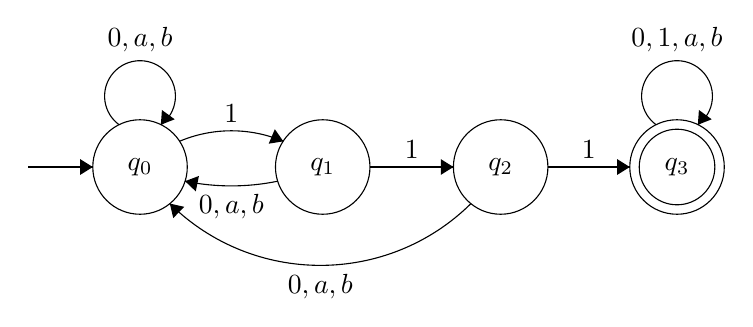
\begin{tikzpicture}[scale=0.2]
\tikzstyle{every node}+=[inner sep=0pt]
\draw [black] (9.5,-31.6) circle (3);
\draw (9.5,-31.6) node {$q_0$};
\draw [black] (21.1,-31.6) circle (3);
\draw (21.1,-31.6) node {$q_1$};
\draw [black] (32.4,-31.6) circle (3);
\draw (32.4,-31.6) node {$q_2$};
\draw [black] (43.6,-31.6) circle (3);
\draw (43.6,-31.6) node {$q_3$};
\draw [black] (43.6,-31.6) circle (2.4);
\draw [black] (2.4,-31.6) -- (6.5,-31.6);
\fill [black] (6.5,-31.6) -- (5.7,-31.1) -- (5.7,-32.1);
\draw [black] (12,-29.97) arc (112.95143:67.04857:8.463);
\fill [black] (18.6,-29.97) -- (18.06,-29.2) -- (17.67,-30.12);
\draw (15.3,-28.8) node [above] {$1$};
\draw [black] (8.177,-28.92) arc (234:-54:2.25);
\draw (9.5,-24.35) node [above] {$0,a,b$};
\fill [black] (10.82,-28.92) -- (11.7,-28.57) -- (10.89,-27.98);
\draw [black] (35.4,-31.6) -- (40.6,-31.6);
\fill [black] (40.6,-31.6) -- (39.8,-31.1) -- (39.8,-32.1);
\draw (38,-31.1) node [above] {$1$};
\draw [black] (42.277,-28.92) arc (234:-54:2.25);
\draw (43.6,-24.35) node [above] {$0,1,a,b$};
\fill [black] (44.92,-28.92) -- (45.8,-28.57) -- (44.99,-27.98);
\draw [black] (18.244,-32.501) arc (-78.37754:-101.62246:14.613);
\fill [black] (12.36,-32.5) -- (13.04,-33.15) -- (13.24,-32.17);
\draw (15.3,-33.3) node [below] {$0,a,b$};
\draw [black] (30.513,-33.924) arc (-45.38469:-134.61531:13.616);
\fill [black] (11.39,-33.92) -- (11.61,-34.84) -- (12.31,-34.13);
\draw (20.95,-38.35) node [below] {$0,a,b$};
\draw [black] (24.1,-31.6) -- (29.4,-31.6);
\fill [black] (29.4,-31.6) -- (28.6,-31.1) -- (28.6,-32.1);
\draw (26.75,-31.1) node [above] {$1$};
\end{tikzpicture}
\end{center}

Akzeptiere $M_2$ die Sprache $L_2 = \mathcal{L}(M_2) = \{ x \in \{0,1,a,b \}^* | x$ enthält das Teilwort $aba \}$:

\begin{center}
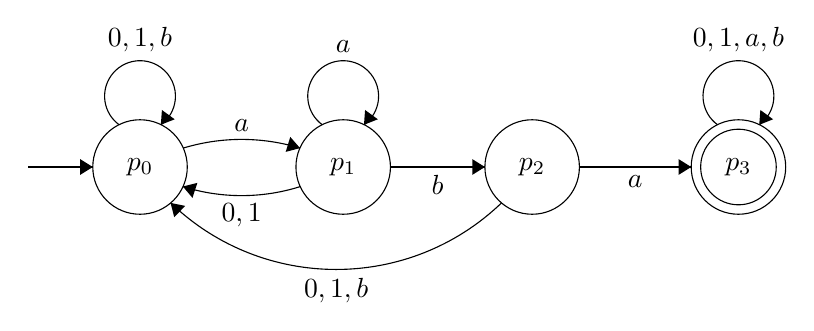
\begin{tikzpicture}[scale=0.2]
\tikzstyle{every node}+=[inner sep=0pt]
\draw [black] (11.5,-28.4) circle (3);
\draw (11.5,-28.4) node {$p_0$};
\draw [black] (24.4,-28.4) circle (3);
\draw (24.4,-28.4) node {$p_1$};
\draw [black] (36.4,-28.4) circle (3);
\draw (36.4,-28.4) node {$p_2$};
\draw [black] (49.5,-28.4) circle (3);
\draw (49.5,-28.4) node {$p_3$};
\draw [black] (49.5,-28.4) circle (2.4);
\draw [black] (4.4,-28.4) -- (8.5,-28.4);
\fill [black] (8.5,-28.4) -- (7.7,-27.9) -- (7.7,-28.9);
\draw [black] (14.242,-27.199) arc (106.91011:73.08989:12.749);
\fill [black] (21.66,-27.2) -- (21.04,-26.49) -- (20.75,-27.44);
\draw (17.95,-26.15) node [above] {$a$};
\draw [black] (27.4,-28.4) -- (33.4,-28.4);
\fill [black] (33.4,-28.4) -- (32.6,-27.9) -- (32.6,-28.9);
\draw (30.4,-28.9) node [below] {$b$};
\draw [black] (39.4,-28.4) -- (46.5,-28.4);
\fill [black] (46.5,-28.4) -- (45.7,-27.9) -- (45.7,-28.9);
\draw (42.95,-28.9) node [below] {$a$};
\draw [black] (10.177,-25.72) arc (234:-54:2.25);
\draw (11.5,-21.15) node [above] {$0,1,b$};
\fill [black] (12.82,-25.72) -- (13.7,-25.37) -- (12.89,-24.78);
\draw [black] (21.677,-29.642) arc (-72.44382:-107.55618:12.356);
\fill [black] (14.22,-29.64) -- (14.83,-30.36) -- (15.14,-29.41);
\draw (17.95,-30.72) node [below] {$0,1$};
\draw [black] (34.456,-30.678) arc (-46.14958:-133.85042:15.164);
\fill [black] (13.44,-30.68) -- (13.67,-31.59) -- (14.37,-30.87);
\draw (23.95,-35.41) node [below] {$0,1,b$};
\draw [black] (48.177,-25.72) arc (234:-54:2.25);
\draw (49.5,-21.15) node [above] {$0,1,a,b$};
\fill [black] (50.82,-25.72) -- (51.7,-25.37) -- (50.89,-24.78);
\draw [black] (23.077,-25.72) arc (234:-54:2.25);
\draw (24.4,-21.15) node [above] {$a$};
\fill [black] (25.72,-25.72) -- (26.6,-25.37) -- (25.79,-24.78);
\end{tikzpicture}
\end{center}

$M$ akzeptiert nun die Sprache $L = \mathcal{L}(M) = L_1 \cup L_2$. Darum ist 
\begin{eqnarray*}
Q_M &=& Q_{M_1} \times Q_{M_2} \\
&=& \{
(q_0, p_0),(q_0, p_1),(q_0, p_2),(q_0, p_3), \\
&&(q_1, p_0),(q_1, p_1),(q_1, p_2),(q_1, p_3), \\
&&(q_2, p_0),(q_2, p_1),(q_2, p_2),(q_2, p_3), \\
&&(q_3, p_0),(q_3, p_1),(q_3, p_2),(q_3, p_3)
\}
\end{eqnarray*}
mit $Q_{M_1} = \{q_0,q_1,q_2,q_3\}$ und $Q_{M_2} = \{p_0,p_1,p_2,p_3\}$. Matrixmässig angeordnet sieht das so aus:

\begin{center}
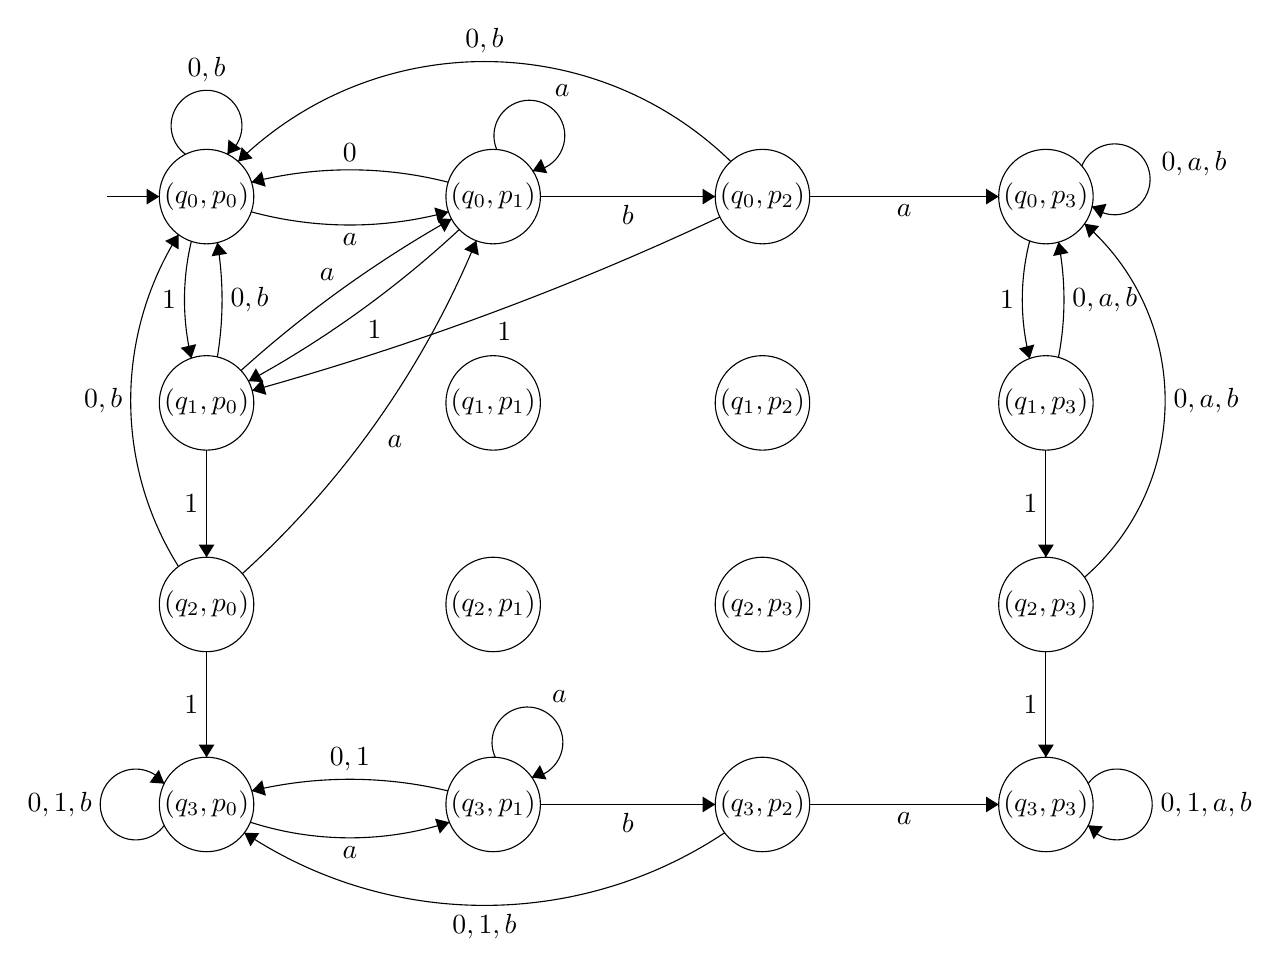
\begin{tikzpicture}[scale=0.2]
\tikzstyle{every node}+=[inner sep=0pt]
\draw [black] (11.6,-11.1) circle (3);
\draw (11.6,-11.1) node {$(q_0,p_0)$};
\draw [black] (29.8,-11.1) circle (3);
\draw (29.8,-11.1) node {$(q_0,p_1)$};
\draw [black] (46.9,-11.1) circle (3);
\draw (46.9,-11.1) node {$(q_0,p_2)$};
\draw [black] (64.9,-11.1) circle (3);
\draw (64.9,-11.1) node {$(q_0,p_3)$};
\draw [black] (11.6,-24.2) circle (3);
\draw (11.6,-24.2) node {$(q_1,p_0)$};
\draw [black] (29.8,-24.2) circle (3);
\draw (29.8,-24.2) node {$(q_1,p_1)$};
\draw [black] (46.9,-24.2) circle (3);
\draw (46.9,-24.2) node {$(q_1,p_2)$};
\draw [black] (64.9,-24.2) circle (3);
\draw (64.9,-24.2) node {$(q_1,p_3)$};
\draw [black] (11.6,-37) circle (3);
\draw (11.6,-37) node {$(q_2,p_0)$};
\draw [black] (29.8,-37) circle (3);
\draw (29.8,-37) node {$(q_2,p_1)$};
\draw [black] (46.9,-37) circle (3);
\draw (46.9,-37) node {$(q_2,p_3)$};
\draw [black] (64.9,-37) circle (3);
\draw (64.9,-37) node {$(q_2,p_3)$};
\draw [black] (11.6,-49.7) circle (3);
\draw (11.6,-49.7) node {$(q_3,p_0)$};
\draw [black] (29.8,-49.7) circle (3);
\draw (29.8,-49.7) node {$(q_3,p_1)$};
\draw [black] (46.9,-49.7) circle (3);
\draw (46.9,-49.7) node {$(q_3,p_2)$};
\draw [black] (64.9,-49.7) circle (3);
\draw (64.9,-49.7) node {$(q_3,p_3)$};
\draw [black] (5.3,-11.1) -- (8.6,-11.1);
\fill [black] (8.6,-11.1) -- (7.8,-10.6) -- (7.8,-11.6);
\draw [black] (10.277,-8.42) arc (234:-54:2.25);
\draw (11.6,-3.85) node [above] {$0,b$};
\fill [black] (12.92,-8.42) -- (13.8,-8.07) -- (12.99,-7.48);
\draw [black] (10.635,-21.364) arc (-166.57921:-193.42079:16.002);
\fill [black] (10.64,-21.36) -- (10.94,-20.47) -- (9.96,-20.7);
\draw (9.7,-17.65) node [left] {$1$};
\draw [black] (26.962,-12.067) arc (-74.78526:-105.21474:23.862);
\fill [black] (26.96,-12.07) -- (26.06,-11.79) -- (26.32,-12.76);
\draw (20.7,-13.4) node [below] {$a$};
\draw [black] (14.455,-10.186) arc (104.34394:75.65606:25.206);
\fill [black] (14.46,-10.19) -- (15.35,-10.47) -- (15.11,-9.5);
\draw (20.7,-8.9) node [above] {$0$};
\draw [black] (27.649,-13.191) arc (-47.10492:-61.40389:66.247);
\fill [black] (14.27,-22.82) -- (15.21,-22.88) -- (14.73,-22);
\draw (22.26,-18.92) node [below] {$1$};
\draw [black] (30.033,-8.121) arc (203.26601:-84.73399:2.25);
\draw (34.19,-4.8) node [above] {$a$};
\fill [black] (32.31,-9.47) -- (33.24,-9.62) -- (32.84,-8.7);
\draw [black] (32.8,-11.1) -- (43.9,-11.1);
\fill [black] (43.9,-11.1) -- (43.1,-10.6) -- (43.1,-11.6);
\draw (38.35,-11.6) node [below] {$b$};
\draw [black] (13.606,-8.872) arc (134.17594:45.82406:22.45);
\fill [black] (13.61,-8.87) -- (14.53,-8.67) -- (13.83,-7.96);
\draw (29.25,-2.02) node [above] {$0,b$};
\draw [black] (44.195,-12.398) arc (-64.81751:-74.46222:188.409);
\fill [black] (14.5,-23.42) -- (15.4,-23.69) -- (15.13,-22.72);
\draw (30.51,-19.06) node [below] {$1$};
\draw [black] (49.9,-11.1) -- (61.9,-11.1);
\fill [black] (61.9,-11.1) -- (61.1,-10.6) -- (61.1,-11.6);
\draw (55.9,-11.6) node [below] {$a$};
\draw [black] (12.287,-14.018) arc (9.39173:-9.39173:22.258);
\fill [black] (12.29,-14.02) -- (11.92,-14.89) -- (12.91,-14.73);
\draw (13.09,-17.65) node [right] {$0,b$};
\draw [black] (11.6,-27.2) -- (11.6,-34);
\fill [black] (11.6,-34) -- (12.1,-33.2) -- (11.1,-33.2);
\draw (11.1,-30.6) node [left] {$1$};
\draw [black] (13.786,-22.145) arc (132.07598:119.4152:74.712);
\fill [black] (27.16,-12.52) -- (26.22,-12.48) -- (26.71,-13.35);
\draw (19.26,-16.47) node [above] {$a$};
\draw [black] (9.818,-34.59) arc (-147.85809:-212.14191:19.812);
\fill [black] (9.82,-13.51) -- (8.97,-13.92) -- (9.82,-14.45);
\draw (6.28,-24.05) node [left] {$0,b$};
\draw [black] (11.6,-40) -- (11.6,-46.7);
\fill [black] (11.6,-46.7) -- (12.1,-45.9) -- (11.1,-45.9);
\draw (11.1,-43.35) node [left] {$1$};
\draw [black] (28.729,-13.902) arc (-22.37867:-47.81296:58.687);
\fill [black] (28.73,-13.9) -- (27.96,-14.45) -- (28.89,-14.83);
\draw (23.07,-26.67) node [right] {$a$};
\draw [black] (8.92,-51.023) arc (324:36:2.25);
\draw (4.35,-49.7) node [left] {$0,1,b$};
\fill [black] (8.92,-48.38) -- (8.57,-47.5) -- (7.98,-48.31);
\draw [black] (27.022,-50.825) arc (-72.12232:-107.87768:20.593);
\fill [black] (27.02,-50.83) -- (26.11,-50.6) -- (26.41,-51.55);
\draw (20.7,-52.32) node [below] {$a$};
\draw [black] (29.939,-46.715) arc (205.07193:-82.92807:2.25);
\draw (34.01,-43.29) node [above] {$a$};
\fill [black] (32.25,-47.99) -- (33.19,-48.11) -- (32.77,-47.2);
\draw [black] (32.8,-49.7) -- (43.9,-49.7);
\fill [black] (43.9,-49.7) -- (43.1,-49.2) -- (43.1,-50.2);
\draw (38.35,-50.2) node [below] {$b$};
\draw [black] (14.471,-48.837) arc (103.50743:76.49257:26.666);
\fill [black] (14.47,-48.84) -- (15.37,-49.14) -- (15.13,-48.16);
\draw (20.7,-47.6) node [above] {$0,1$};
\draw [black] (49.9,-49.7) -- (61.9,-49.7);
\fill [black] (61.9,-49.7) -- (61.1,-49.2) -- (61.1,-50.2);
\draw (55.9,-50.2) node [below] {$a$};
\draw [black] (44.499,-51.496) arc (-56.33345:-123.66655:27.507);
\fill [black] (14,-51.5) -- (14.39,-52.36) -- (14.94,-51.52);
\draw (29.25,-56.61) node [below] {$0,1,b$};
\draw [black] (67.58,-48.377) arc (144:-144:2.25);
\draw (72.15,-49.7) node [right] {$0,1,a,b$};
\fill [black] (67.58,-51.02) -- (67.93,-51.9) -- (68.52,-51.09);
\draw [black] (67.177,-9.164) arc (158.10199:-129.89801:2.25);
\draw (72.21,-8.99) node [right] {$0,a,b$};
\fill [black] (67.82,-11.73) -- (68.38,-12.49) -- (68.75,-11.56);
\draw [black] (63.871,-21.387) arc (-165.61565:-194.38435:15.044);
\fill [black] (63.87,-21.39) -- (64.16,-20.49) -- (63.19,-20.74);
\draw (62.9,-17.65) node [left] {$1$};
\draw [black] (65.696,-13.989) arc (10.95119:-10.95119:19.27);
\fill [black] (65.7,-13.99) -- (65.36,-14.87) -- (66.34,-14.68);
\draw (66.55,-17.65) node [right] {$0,a,b$};
\draw [black] (64.9,-27.2) -- (64.9,-34);
\fill [black] (64.9,-34) -- (65.4,-33.2) -- (64.4,-33.2);
\draw (64.4,-30.6) node [left] {$1$};
\draw [black] (67.348,-12.825) arc (49.05694:-49.05694:14.861);
\fill [black] (67.35,-12.82) -- (67.63,-13.73) -- (68.28,-12.97);
\draw (72.97,-24.05) node [right] {$0,a,b$};
\draw [black] (64.9,-40) -- (64.9,-46.7);
\fill [black] (64.9,-46.7) -- (65.4,-45.9) -- (64.4,-45.9);
\draw (64.4,-43.35) node [left] {$1$};
\end{tikzpicture}
\end{center}

Nach Entfernung der unerreichbaren Zustände und Markierung der akzeptierenden Zustände
\[
F_M = (F_{M_1} \times Q_{M_2}) \cup (Q_{M_1} \times F_{M_2})
\]

erhalten wir:

\begin{center}
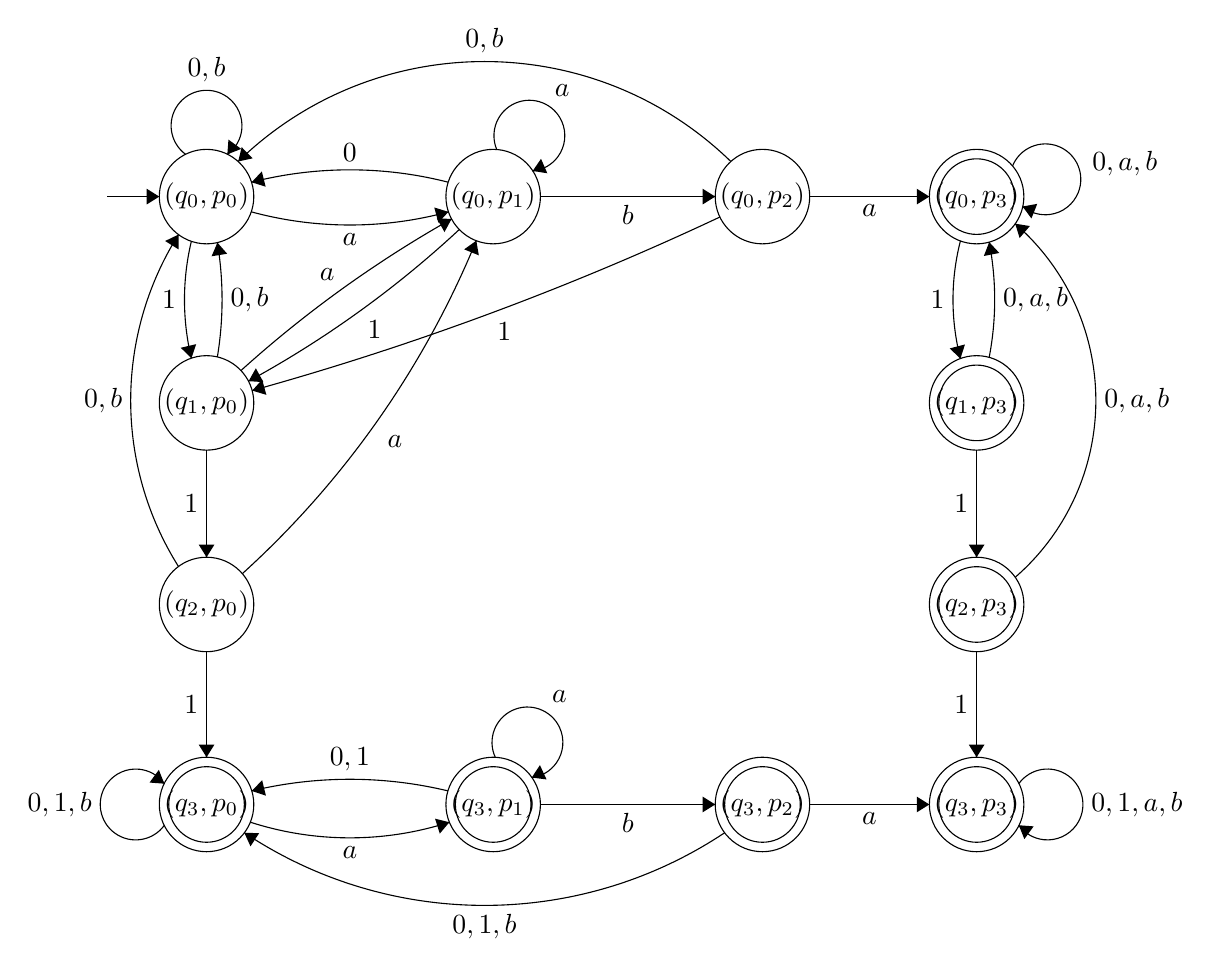
\begin{tikzpicture}[scale=0.2]
\tikzstyle{every node}+=[inner sep=0pt]
\draw [black] (11.6,-11.1) circle (3);
\draw (11.6,-11.1) node {$(q_0,p_0)$};
\draw [black] (29.8,-11.1) circle (3);
\draw (29.8,-11.1) node {$(q_0,p_1)$};
\draw [black] (46.9,-11.1) circle (3);
\draw (46.9,-11.1) node {$(q_0,p_2)$};
\draw [black] (60.5,-11.1) circle (3);
\draw (60.5,-11.1) node {$(q_0,p_3)$};
\draw [black] (60.5,-11.1) circle (2.4);
\draw [black] (11.6,-24.2) circle (3);
\draw (11.6,-24.2) node {$(q_1,p_0)$};
\draw [black] (60.5,-24.2) circle (3);
\draw (60.5,-24.2) node {$(q_1,p_3)$};
\draw [black] (60.5,-24.2) circle (2.4);
\draw [black] (11.6,-37) circle (3);
\draw (11.6,-37) node {$(q_2,p_0)$};
\draw [black] (60.5,-37) circle (3);
\draw (60.5,-37) node {$(q_2,p_3)$};
\draw [black] (60.5,-37) circle (2.4);
\draw [black] (11.6,-49.7) circle (3);
\draw (11.6,-49.7) node {$(q_3,p_0)$};
\draw [black] (11.6,-49.7) circle (2.4);
\draw [black] (29.8,-49.7) circle (3);
\draw (29.8,-49.7) node {$(q_3,p_1)$};
\draw [black] (29.8,-49.7) circle (2.4);
\draw [black] (46.9,-49.7) circle (3);
\draw (46.9,-49.7) node {$(q_3,p_2)$};
\draw [black] (46.9,-49.7) circle (2.4);
\draw [black] (60.5,-49.7) circle (3);
\draw (60.5,-49.7) node {$(q_3,p_3)$};
\draw [black] (60.5,-49.7) circle (2.4);
\draw [black] (5.3,-11.1) -- (8.6,-11.1);
\fill [black] (8.6,-11.1) -- (7.8,-10.6) -- (7.8,-11.6);
\draw [black] (10.277,-8.42) arc (234:-54:2.25);
\draw (11.6,-3.85) node [above] {$0,b$};
\fill [black] (12.92,-8.42) -- (13.8,-8.07) -- (12.99,-7.48);
\draw [black] (10.635,-21.364) arc (-166.57921:-193.42079:16.002);
\fill [black] (10.64,-21.36) -- (10.94,-20.47) -- (9.96,-20.7);
\draw (9.7,-17.65) node [left] {$1$};
\draw [black] (26.962,-12.067) arc (-74.78526:-105.21474:23.862);
\fill [black] (26.96,-12.07) -- (26.06,-11.79) -- (26.32,-12.76);
\draw (20.7,-13.4) node [below] {$a$};
\draw [black] (14.455,-10.186) arc (104.34394:75.65606:25.206);
\fill [black] (14.46,-10.19) -- (15.35,-10.47) -- (15.11,-9.5);
\draw (20.7,-8.9) node [above] {$0$};
\draw [black] (27.649,-13.191) arc (-47.10492:-61.40389:66.247);
\fill [black] (14.27,-22.82) -- (15.21,-22.88) -- (14.73,-22);
\draw (22.26,-18.92) node [below] {$1$};
\draw [black] (30.033,-8.121) arc (203.26601:-84.73399:2.25);
\draw (34.19,-4.8) node [above] {$a$};
\fill [black] (32.31,-9.47) -- (33.24,-9.62) -- (32.84,-8.7);
\draw [black] (32.8,-11.1) -- (43.9,-11.1);
\fill [black] (43.9,-11.1) -- (43.1,-10.6) -- (43.1,-11.6);
\draw (38.35,-11.6) node [below] {$b$};
\draw [black] (13.606,-8.872) arc (134.17594:45.82406:22.45);
\fill [black] (13.61,-8.87) -- (14.53,-8.67) -- (13.83,-7.96);
\draw (29.25,-2.02) node [above] {$0,b$};
\draw [black] (44.195,-12.398) arc (-64.81751:-74.46222:188.409);
\fill [black] (14.5,-23.42) -- (15.4,-23.69) -- (15.13,-22.72);
\draw (30.51,-19.06) node [below] {$1$};
\draw [black] (49.9,-11.1) -- (57.5,-11.1);
\fill [black] (57.5,-11.1) -- (56.7,-10.6) -- (56.7,-11.6);
\draw (53.7,-11.6) node [below] {$a$};
\draw [black] (12.287,-14.018) arc (9.39173:-9.39173:22.258);
\fill [black] (12.29,-14.02) -- (11.92,-14.89) -- (12.91,-14.73);
\draw (13.09,-17.65) node [right] {$0,b$};
\draw [black] (11.6,-27.2) -- (11.6,-34);
\fill [black] (11.6,-34) -- (12.1,-33.2) -- (11.1,-33.2);
\draw (11.1,-30.6) node [left] {$1$};
\draw [black] (13.786,-22.145) arc (132.07598:119.4152:74.712);
\fill [black] (27.16,-12.52) -- (26.22,-12.48) -- (26.71,-13.35);
\draw (19.26,-16.47) node [above] {$a$};
\draw [black] (9.818,-34.59) arc (-147.85809:-212.14191:19.812);
\fill [black] (9.82,-13.51) -- (8.97,-13.92) -- (9.82,-14.45);
\draw (6.28,-24.05) node [left] {$0,b$};
\draw [black] (11.6,-40) -- (11.6,-46.7);
\fill [black] (11.6,-46.7) -- (12.1,-45.9) -- (11.1,-45.9);
\draw (11.1,-43.35) node [left] {$1$};
\draw [black] (28.729,-13.902) arc (-22.37867:-47.81296:58.687);
\fill [black] (28.73,-13.9) -- (27.96,-14.45) -- (28.89,-14.83);
\draw (23.07,-26.67) node [right] {$a$};
\draw [black] (8.92,-51.023) arc (324:36:2.25);
\draw (4.35,-49.7) node [left] {$0,1,b$};
\fill [black] (8.92,-48.38) -- (8.57,-47.5) -- (7.98,-48.31);
\draw [black] (27.022,-50.825) arc (-72.12232:-107.87768:20.593);
\fill [black] (27.02,-50.83) -- (26.11,-50.6) -- (26.41,-51.55);
\draw (20.7,-52.32) node [below] {$a$};
\draw [black] (29.939,-46.715) arc (205.07193:-82.92807:2.25);
\draw (34.01,-43.29) node [above] {$a$};
\fill [black] (32.25,-47.99) -- (33.19,-48.11) -- (32.77,-47.2);
\draw [black] (32.8,-49.7) -- (43.9,-49.7);
\fill [black] (43.9,-49.7) -- (43.1,-49.2) -- (43.1,-50.2);
\draw (38.35,-50.2) node [below] {$b$};
\draw [black] (14.471,-48.837) arc (103.50743:76.49257:26.666);
\fill [black] (14.47,-48.84) -- (15.37,-49.14) -- (15.13,-48.16);
\draw (20.7,-47.6) node [above] {$0,1$};
\draw [black] (49.9,-49.7) -- (57.5,-49.7);
\fill [black] (57.5,-49.7) -- (56.7,-49.2) -- (56.7,-50.2);
\draw (53.7,-50.2) node [below] {$a$};
\draw [black] (44.499,-51.496) arc (-56.33345:-123.66655:27.507);
\fill [black] (14,-51.5) -- (14.39,-52.36) -- (14.94,-51.52);
\draw (29.25,-56.61) node [below] {$0,1,b$};
\draw [black] (63.18,-48.377) arc (144:-144:2.25);
\draw (67.75,-49.7) node [right] {$0,1,a,b$};
\fill [black] (63.18,-51.02) -- (63.53,-51.9) -- (64.12,-51.09);
\draw [black] (62.777,-9.164) arc (158.10199:-129.89801:2.25);
\draw (67.81,-8.99) node [right] {$0,a,b$};
\fill [black] (63.42,-11.73) -- (63.98,-12.49) -- (64.35,-11.56);
\draw [black] (59.471,-21.387) arc (-165.61565:-194.38435:15.044);
\fill [black] (59.47,-21.39) -- (59.76,-20.49) -- (58.79,-20.74);
\draw (58.5,-17.65) node [left] {$1$};
\draw [black] (61.296,-13.989) arc (10.95119:-10.95119:19.27);
\fill [black] (61.3,-13.99) -- (60.96,-14.87) -- (61.94,-14.68);
\draw (62.15,-17.65) node [right] {$0,a,b$};
\draw [black] (60.5,-27.2) -- (60.5,-34);
\fill [black] (60.5,-34) -- (61,-33.2) -- (60,-33.2);
\draw (60,-30.6) node [left] {$1$};
\draw [black] (62.948,-12.825) arc (49.05694:-49.05694:14.861);
\fill [black] (62.95,-12.82) -- (63.23,-13.73) -- (63.88,-12.97);
\draw (68.57,-24.05) node [right] {$0,a,b$};
\draw [black] (60.5,-40) -- (60.5,-46.7);
\fill [black] (60.5,-46.7) -- (61,-45.9) -- (60,-45.9);
\draw (60,-43.35) node [left] {$1$};
\end{tikzpicture}
\end{center}


\section*{Aufgabe 6.2(j)}

Akzeptiere $M_1$ die Sprache $L_1 = \mathcal{L}(M_1) = \{x \in \{0,1\}^* | x $ enthält das Teilwort 0011$ \}$:

\begin{center}
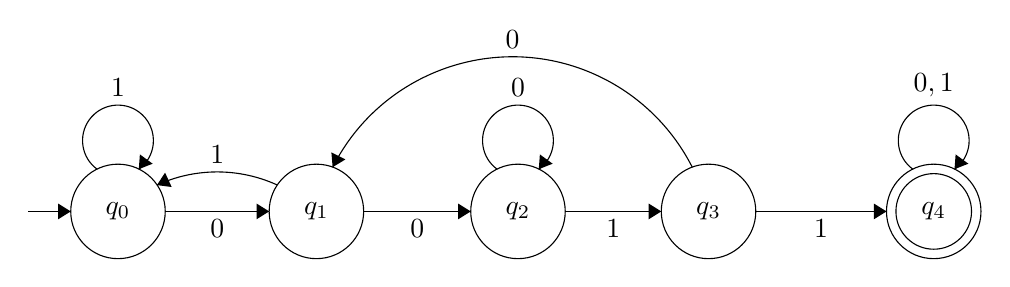
\begin{tikzpicture}[scale=0.2]
\tikzstyle{every node}+=[inner sep=0pt]
\draw [black] (10.5,-14.1) circle (3);
\draw (10.5,-14.1) node {$q_0$};
\draw [black] (23.1,-14.1) circle (3);
\draw (23.1,-14.1) node {$q_1$};
\draw [black] (35.9,-14.1) circle (3);
\draw (35.9,-14.1) node {$q_2$};
\draw [black] (48,-14.1) circle (3);
\draw (48,-14.1) node {$q_3$};
\draw [black] (62.3,-14.1) circle (3);
\draw (62.3,-14.1) node {$q_4$};
\draw [black] (62.3,-14.1) circle (2.4);
\draw [black] (4.8,-14.1) -- (7.5,-14.1);
\fill [black] (7.5,-14.1) -- (6.7,-13.6) -- (6.7,-14.6);
\draw [black] (13.5,-14.1) -- (20.1,-14.1);
\fill [black] (20.1,-14.1) -- (19.3,-13.6) -- (19.3,-14.6);
\draw (16.8,-14.6) node [below] {$0$};
\draw [black] (9.177,-11.42) arc (234:-54:2.25);
\draw (10.5,-6.85) node [above] {$1$};
\fill [black] (11.82,-11.42) -- (12.7,-11.07) -- (11.89,-10.48);
\draw [black] (26.1,-14.1) -- (32.9,-14.1);
\fill [black] (32.9,-14.1) -- (32.1,-13.6) -- (32.1,-14.6);
\draw (29.5,-14.6) node [below] {$0$};
\draw [black] (12.975,-12.428) arc (114.67074:65.32926:9.165);
\fill [black] (12.97,-12.43) -- (13.91,-12.55) -- (13.49,-11.64);
\draw (16.8,-11.09) node [above] {$1$};
\draw [black] (38.9,-14.1) -- (45,-14.1);
\fill [black] (45,-14.1) -- (44.2,-13.6) -- (44.2,-14.6);
\draw (41.95,-14.6) node [below] {$1$};
\draw [black] (51,-14.1) -- (59.3,-14.1);
\fill [black] (59.3,-14.1) -- (58.5,-13.6) -- (58.5,-14.6);
\draw (55.15,-14.6) node [below] {$1$};
\draw [black] (34.577,-11.42) arc (234:-54:2.25);
\draw (35.9,-6.85) node [above] {$0$};
\fill [black] (37.22,-11.42) -- (38.1,-11.07) -- (37.29,-10.48);
\draw [black] (24.133,-11.291) arc (153.10175:26.89825:12.802);
\fill [black] (24.13,-11.29) -- (24.94,-10.8) -- (24.05,-10.35);
\draw (35.55,-3.78) node [above] {$0$};
\draw [black] (60.977,-11.42) arc (234:-54:2.25);
\draw (62.3,-6.85) node [above] {$0,1$};
\fill [black] (63.62,-11.42) -- (64.5,-11.07) -- (63.69,-10.48);
\end{tikzpicture}
\end{center}

Akzeptiere $M_2$ die Sprache $L_2 = \mathcal{L}(M_2) = \{x \in \{0,1\}^* | x $ enthält das Teilwort 110$ \}$:

\begin{center}
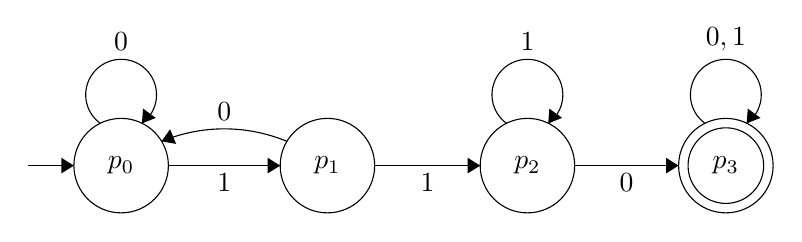
\begin{tikzpicture}[scale=0.2]
\tikzstyle{every node}+=[inner sep=0pt]
\draw [black] (10.6,-16) circle (3);
\draw (10.6,-16) node {$p_0$};
\draw [black] (23.7,-16) circle (3);
\draw (23.7,-16) node {$p_1$};
\draw [black] (36.4,-16) circle (3);
\draw (36.4,-16) node {$p_2$};
\draw [black] (49,-16) circle (3);
\draw (49,-16) node {$p_3$};
\draw [black] (49,-16) circle (2.4);
\draw [black] (4.7,-16) -- (7.6,-16);
\fill [black] (7.6,-16) -- (6.8,-15.5) -- (6.8,-16.5);
\draw [black] (13.6,-16) -- (20.7,-16);
\fill [black] (20.7,-16) -- (19.9,-15.5) -- (19.9,-16.5);
\draw (17.15,-16.5) node [below] {$1$};
\draw [black] (26.7,-16) -- (33.4,-16);
\fill [black] (33.4,-16) -- (32.6,-15.5) -- (32.6,-16.5);
\draw (30.05,-16.5) node [below] {$1$};
\draw [black] (39.4,-16) -- (46,-16);
\fill [black] (46,-16) -- (45.2,-15.5) -- (45.2,-16.5);
\draw (42.7,-16.5) node [below] {$0$};
\draw [black] (9.277,-13.32) arc (234:-54:2.25);
\draw (10.6,-8.75) node [above] {$0$};
\fill [black] (11.92,-13.32) -- (12.8,-12.97) -- (11.99,-12.38);
\draw [black] (13.164,-14.463) arc (112.64008:67.35992:10.355);
\fill [black] (13.16,-14.46) -- (14.09,-14.62) -- (13.71,-13.69);
\draw (17.15,-13.17) node [above] {$0$};
\draw [black] (47.677,-13.32) arc (234:-54:2.25);
\draw (49,-8.75) node [above] {$0,1$};
\fill [black] (50.32,-13.32) -- (51.2,-12.97) -- (50.39,-12.38);
\draw [black] (35.077,-13.32) arc (234:-54:2.25);
\draw (36.4,-8.75) node [above] {$1$};
\fill [black] (37.72,-13.32) -- (38.6,-12.97) -- (37.79,-12.38);
\end{tikzpicture}
\end{center}

Es folgt die nämliche Konstruktion mit $L_M = \mathcal{L}(M) = L_1 \cup L_2$:

\begin{center}
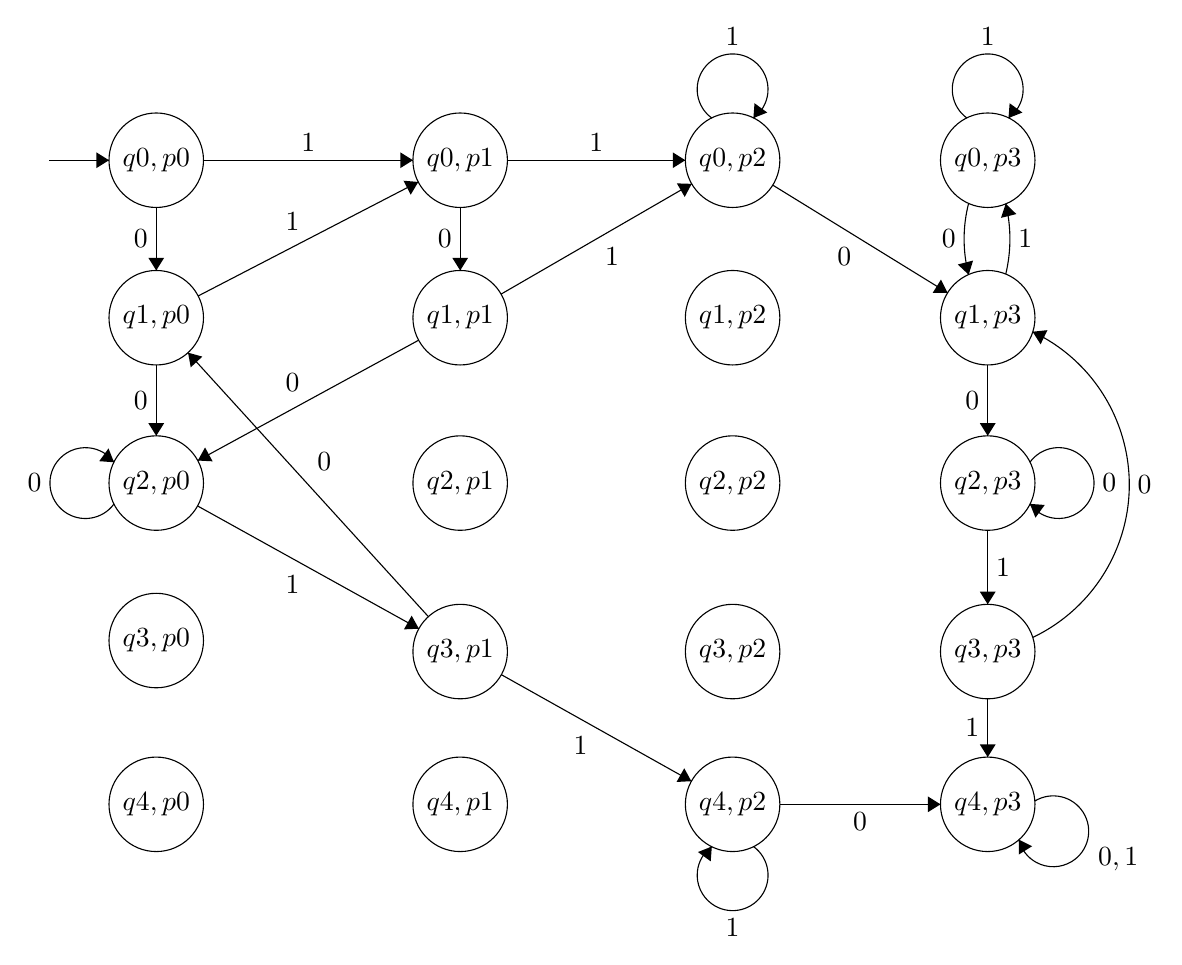
\begin{tikzpicture}[scale=0.2]
\tikzstyle{every node}+=[inner sep=0pt]
\draw [black] (11,-9.3) circle (3);
\draw (11,-9.3) node {$q0,p0$};
\draw [black] (30.3,-9.3) circle (3);
\draw (30.3,-9.3) node {$q0,p1$};
\draw [black] (47.6,-9.3) circle (3);
\draw (47.6,-9.3) node {$q0,p2$};
\draw [black] (63.8,-9.3) circle (3);
\draw (63.8,-9.3) node {$q0,p3$};
\draw [black] (11,-19.3) circle (3);
\draw (11,-19.3) node {$q1,p0$};
\draw [black] (11,-29.8) circle (3);
\draw (11,-29.8) node {$q2,p0$};
\draw [black] (30.3,-29.8) circle (3);
\draw (30.3,-29.8) node {$q2,p1$};
\draw [black] (47.6,-29.8) circle (3);
\draw (47.6,-29.8) node {$q2,p2$};
\draw [black] (63.8,-29.8) circle (3);
\draw (63.8,-29.8) node {$q2,p3$};
\draw [black] (30.3,-19.3) circle (3);
\draw (30.3,-19.3) node {$q1,p1$};
\draw [black] (11,-39.8) circle (3);
\draw (11,-39.8) node {$q3,p0$};
\draw [black] (30.3,-40.5) circle (3);
\draw (30.3,-40.5) node {$q3,p1$};
\draw [black] (47.6,-40.5) circle (3);
\draw (47.6,-40.5) node {$q3,p2$};
\draw [black] (63.8,-40.5) circle (3);
\draw (63.8,-40.5) node {$q3,p3$};
\draw [black] (47.6,-19.3) circle (3);
\draw (47.6,-19.3) node {$q1,p2$};
\draw [black] (11,-50.2) circle (3);
\draw (11,-50.2) node {$q4,p0$};
\draw [black] (30.3,-50.2) circle (3);
\draw (30.3,-50.2) node {$q4,p1$};
\draw [black] (47.6,-50.2) circle (3);
\draw (47.6,-50.2) node {$q4,p2$};
\draw [black] (63.8,-50.2) circle (3);
\draw (63.8,-50.2) node {$q4,p3$};
\draw [black] (63.8,-19.3) circle (3);
\draw (63.8,-19.3) node {$q1,p3$};
\draw [black] (11,-12.3) -- (11,-16.3);
\fill [black] (11,-16.3) -- (11.5,-15.5) -- (10.5,-15.5);
\draw (10.5,-14.3) node [left] {$0$};
\draw [black] (14,-9.3) -- (27.3,-9.3);
\fill [black] (27.3,-9.3) -- (26.5,-8.8) -- (26.5,-9.8);
\draw (20.65,-8.8) node [above] {$1$};
\draw [black] (30.3,-12.3) -- (30.3,-16.3);
\fill [black] (30.3,-16.3) -- (30.8,-15.5) -- (29.8,-15.5);
\draw (29.8,-14.3) node [left] {$0$};
\draw [black] (33.3,-9.3) -- (44.6,-9.3);
\fill [black] (44.6,-9.3) -- (43.8,-8.8) -- (43.8,-9.8);
\draw (38.95,-8.8) node [above] {$1$};
\draw [black] (50.15,-10.88) -- (61.25,-17.72);
\fill [black] (61.25,-17.72) -- (60.83,-16.88) -- (60.3,-17.73);
\draw (54.7,-14.8) node [below] {$0$};
\draw [black] (46.277,-6.62) arc (234:-54:2.25);
\draw (47.6,-2.05) node [above] {$1$};
\fill [black] (48.92,-6.62) -- (49.8,-6.27) -- (48.99,-5.68);
\draw [black] (11,-22.3) -- (11,-26.8);
\fill [black] (11,-26.8) -- (11.5,-26) -- (10.5,-26);
\draw (10.5,-24.55) node [left] {$0$};
\draw [black] (13.66,-17.92) -- (27.64,-10.68);
\fill [black] (27.64,-10.68) -- (26.7,-10.6) -- (27.16,-11.49);
\draw (19.66,-13.8) node [above] {$1$};
\draw [black] (27.66,-20.73) -- (13.64,-28.37);
\fill [black] (13.64,-28.37) -- (14.58,-28.42) -- (14.1,-27.54);
\draw (19.65,-24.05) node [above] {$0$};
\draw [black] (32.9,-17.8) -- (45,-10.8);
\fill [black] (45,-10.8) -- (44.06,-10.77) -- (44.56,-11.63);
\draw (39.95,-14.8) node [below] {$1$};
\draw [black] (63.8,-22.3) -- (63.8,-26.8);
\fill [black] (63.8,-26.8) -- (64.3,-26) -- (63.3,-26);
\draw (63.3,-24.55) node [left] {$0$};
\draw [black] (64.943,-12.061) arc (13.51925:-13.51925:9.58);
\fill [black] (64.94,-12.06) -- (64.64,-12.96) -- (65.62,-12.72);
\draw (65.71,-14.3) node [right] {$1$};
\draw [black] (62.477,-6.62) arc (234:-54:2.25);
\draw (63.8,-2.05) node [above] {$1$};
\fill [black] (65.12,-6.62) -- (66,-6.27) -- (65.19,-5.68);
\draw [black] (62.588,-16.571) arc (-165.51911:-194.48089:9.081);
\fill [black] (62.59,-16.57) -- (62.87,-15.67) -- (61.9,-15.92);
\draw (61.8,-14.3) node [left] {$0$};
\draw [black] (8.32,-31.123) arc (324:36:2.25);
\draw (3.75,-29.8) node [left] {$0$};
\fill [black] (8.32,-28.48) -- (7.97,-27.6) -- (7.38,-28.41);
\draw [black] (13.62,-31.25) -- (27.68,-39.05);
\fill [black] (27.68,-39.05) -- (27.22,-38.22) -- (26.73,-39.09);
\draw (19.65,-35.65) node [below] {$1$};
\draw [black] (66.48,-28.477) arc (144:-144:2.25);
\draw (71.05,-29.8) node [right] {$0$};
\fill [black] (66.48,-31.12) -- (66.83,-32) -- (67.42,-31.19);
\draw [black] (63.8,-32.8) -- (63.8,-37.5);
\fill [black] (63.8,-37.5) -- (64.3,-36.7) -- (63.3,-36.7);
\draw (64.3,-35.15) node [right] {$1$};
\draw [black] (28.28,-38.28) -- (13.02,-21.52);
\fill [black] (13.02,-21.52) -- (13.19,-22.45) -- (13.93,-21.77);
\draw (21.19,-28.44) node [right] {$0$};
\draw [black] (32.92,-41.97) -- (44.98,-48.73);
\fill [black] (44.98,-48.73) -- (44.53,-47.91) -- (44.04,-48.78);
\draw (37.95,-45.85) node [below] {$1$};
\draw [black] (66.653,-20.195) arc (64.59164:-64.59164:10.745);
\fill [black] (66.65,-20.19) -- (67.16,-20.99) -- (67.59,-20.09);
\draw (73.29,-29.9) node [right] {$0$};
\draw [black] (63.8,-43.5) -- (63.8,-47.2);
\fill [black] (63.8,-47.2) -- (64.3,-46.4) -- (63.3,-46.4);
\draw (63.3,-45.35) node [left] {$1$};
\draw [black] (48.923,-52.88) arc (54:-234:2.25);
\draw (47.6,-57.45) node [below] {$1$};
\fill [black] (46.28,-52.88) -- (45.4,-53.23) -- (46.21,-53.82);
\draw [black] (50.6,-50.2) -- (60.8,-50.2);
\fill [black] (60.8,-50.2) -- (60,-49.7) -- (60,-50.7);
\draw (55.7,-50.7) node [below] {$0$};
\draw [black] (66.781,-49.997) arc (121.61986:-166.38014:2.25);
\draw (70.78,-53.68) node [right] {$0,1$};
\fill [black] (65.77,-52.44) -- (65.77,-53.39) -- (66.62,-52.86);
\draw [black] (4.2,-9.3) -- (8,-9.3);
\fill [black] (8,-9.3) -- (7.2,-8.8) -- (7.2,-9.8);
\end{tikzpicture}
\end{center}

Und dito mit Endzuständen und ohne unerreichbare Zustände (interessanterweise sind nicht alle Endzustände erreichbar; dies liegt daran, dass beide Wörter je gegenseitige Präfix/Suffix-Kombinationen haben):

\begin{center}
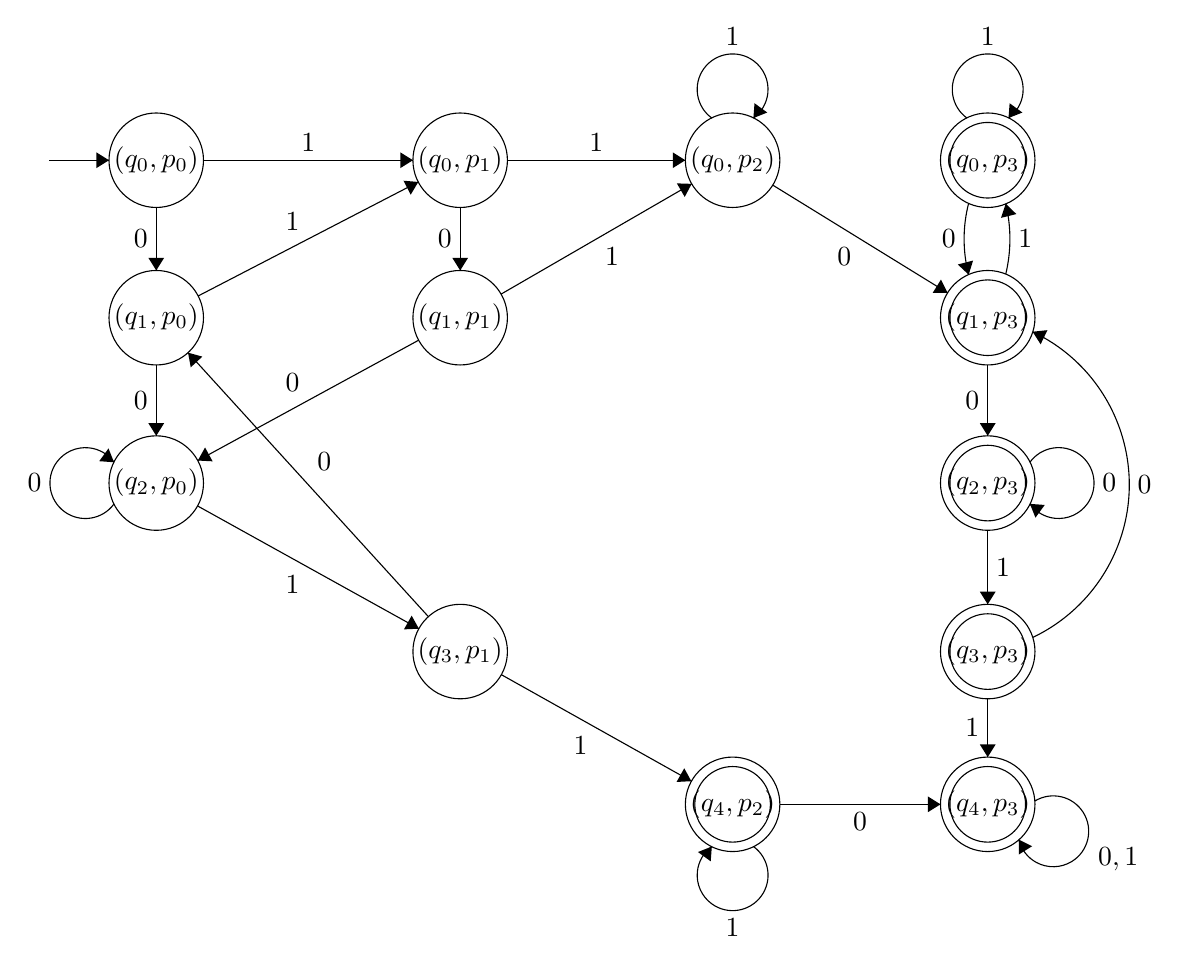
\begin{tikzpicture}[scale=0.2]
\tikzstyle{every node}+=[inner sep=0pt]
\draw [black] (11,-9.3) circle (3);
\draw (11,-9.3) node {$(q_0,p_0)$};
\draw [black] (30.3,-9.3) circle (3);
\draw (30.3,-9.3) node {$(q_0,p_1)$};
\draw [black] (47.6,-9.3) circle (3);
\draw (47.6,-9.3) node {$(q_0,p_2)$};
\draw [black] (63.8,-9.3) circle (3);
\draw (63.8,-9.3) node {$(q_0,p_3)$};
\draw [black] (63.8,-9.3) circle (2.4);
\draw [black] (11,-19.3) circle (3);
\draw (11,-19.3) node {$(q_1,p_0)$};
\draw [black] (11,-29.8) circle (3);
\draw (11,-29.8) node {$(q_2,p_0)$};
\draw [black] (63.8,-29.8) circle (3);
\draw (63.8,-29.8) node {$(q_2,p_3)$};
\draw [black] (63.8,-29.8) circle (2.4);
\draw [black] (30.3,-19.3) circle (3);
\draw (30.3,-19.3) node {$(q_1,p_1)$};
\draw [black] (30.3,-40.5) circle (3);
\draw (30.3,-40.5) node {$(q_3,p_1)$};
\draw [black] (63.8,-40.5) circle (3);
\draw (63.8,-40.5) node {$(q_3,p_3)$};
\draw [black] (63.8,-40.5) circle (2.4);
\draw [black] (47.6,-50.2) circle (3);
\draw (47.6,-50.2) node {$(q_4,p_2)$};
\draw [black] (47.6,-50.2) circle (2.4);
\draw [black] (63.8,-50.2) circle (3);
\draw (63.8,-50.2) node {$(q_4,p_3)$};
\draw [black] (63.8,-50.2) circle (2.4);
\draw [black] (63.8,-19.3) circle (3);
\draw (63.8,-19.3) node {$(q_1,p_3)$};
\draw [black] (63.8,-19.3) circle (2.4);
\draw [black] (11,-12.3) -- (11,-16.3);
\fill [black] (11,-16.3) -- (11.5,-15.5) -- (10.5,-15.5);
\draw (10.5,-14.3) node [left] {$0$};
\draw [black] (14,-9.3) -- (27.3,-9.3);
\fill [black] (27.3,-9.3) -- (26.5,-8.8) -- (26.5,-9.8);
\draw (20.65,-8.8) node [above] {$1$};
\draw [black] (30.3,-12.3) -- (30.3,-16.3);
\fill [black] (30.3,-16.3) -- (30.8,-15.5) -- (29.8,-15.5);
\draw (29.8,-14.3) node [left] {$0$};
\draw [black] (33.3,-9.3) -- (44.6,-9.3);
\fill [black] (44.6,-9.3) -- (43.8,-8.8) -- (43.8,-9.8);
\draw (38.95,-8.8) node [above] {$1$};
\draw [black] (50.15,-10.88) -- (61.25,-17.72);
\fill [black] (61.25,-17.72) -- (60.83,-16.88) -- (60.3,-17.73);
\draw (54.7,-14.8) node [below] {$0$};
\draw [black] (46.277,-6.62) arc (234:-54:2.25);
\draw (47.6,-2.05) node [above] {$1$};
\fill [black] (48.92,-6.62) -- (49.8,-6.27) -- (48.99,-5.68);
\draw [black] (11,-22.3) -- (11,-26.8);
\fill [black] (11,-26.8) -- (11.5,-26) -- (10.5,-26);
\draw (10.5,-24.55) node [left] {$0$};
\draw [black] (13.66,-17.92) -- (27.64,-10.68);
\fill [black] (27.64,-10.68) -- (26.7,-10.6) -- (27.16,-11.49);
\draw (19.66,-13.8) node [above] {$1$};
\draw [black] (27.66,-20.73) -- (13.64,-28.37);
\fill [black] (13.64,-28.37) -- (14.58,-28.42) -- (14.1,-27.54);
\draw (19.65,-24.05) node [above] {$0$};
\draw [black] (32.9,-17.8) -- (45,-10.8);
\fill [black] (45,-10.8) -- (44.06,-10.77) -- (44.56,-11.63);
\draw (39.95,-14.8) node [below] {$1$};
\draw [black] (63.8,-22.3) -- (63.8,-26.8);
\fill [black] (63.8,-26.8) -- (64.3,-26) -- (63.3,-26);
\draw (63.3,-24.55) node [left] {$0$};
\draw [black] (64.943,-12.061) arc (13.51925:-13.51925:9.58);
\fill [black] (64.94,-12.06) -- (64.64,-12.96) -- (65.62,-12.72);
\draw (65.71,-14.3) node [right] {$1$};
\draw [black] (62.477,-6.62) arc (234:-54:2.25);
\draw (63.8,-2.05) node [above] {$1$};
\fill [black] (65.12,-6.62) -- (66,-6.27) -- (65.19,-5.68);
\draw [black] (62.588,-16.571) arc (-165.51911:-194.48089:9.081);
\fill [black] (62.59,-16.57) -- (62.87,-15.67) -- (61.9,-15.92);
\draw (61.8,-14.3) node [left] {$0$};
\draw [black] (8.32,-31.123) arc (324:36:2.25);
\draw (3.75,-29.8) node [left] {$0$};
\fill [black] (8.32,-28.48) -- (7.97,-27.6) -- (7.38,-28.41);
\draw [black] (13.62,-31.25) -- (27.68,-39.05);
\fill [black] (27.68,-39.05) -- (27.22,-38.22) -- (26.73,-39.09);
\draw (19.65,-35.65) node [below] {$1$};
\draw [black] (66.48,-28.477) arc (144:-144:2.25);
\draw (71.05,-29.8) node [right] {$0$};
\fill [black] (66.48,-31.12) -- (66.83,-32) -- (67.42,-31.19);
\draw [black] (63.8,-32.8) -- (63.8,-37.5);
\fill [black] (63.8,-37.5) -- (64.3,-36.7) -- (63.3,-36.7);
\draw (64.3,-35.15) node [right] {$1$};
\draw [black] (28.28,-38.28) -- (13.02,-21.52);
\fill [black] (13.02,-21.52) -- (13.19,-22.45) -- (13.93,-21.77);
\draw (21.19,-28.44) node [right] {$0$};
\draw [black] (32.92,-41.97) -- (44.98,-48.73);
\fill [black] (44.98,-48.73) -- (44.53,-47.91) -- (44.04,-48.78);
\draw (37.95,-45.85) node [below] {$1$};
\draw [black] (66.653,-20.195) arc (64.59164:-64.59164:10.745);
\fill [black] (66.65,-20.19) -- (67.16,-20.99) -- (67.59,-20.09);
\draw (73.29,-29.9) node [right] {$0$};
\draw [black] (63.8,-43.5) -- (63.8,-47.2);
\fill [black] (63.8,-47.2) -- (64.3,-46.4) -- (63.3,-46.4);
\draw (63.3,-45.35) node [left] {$1$};
\draw [black] (48.923,-52.88) arc (54:-234:2.25);
\draw (47.6,-57.45) node [below] {$1$};
\fill [black] (46.28,-52.88) -- (45.4,-53.23) -- (46.21,-53.82);
\draw [black] (50.6,-50.2) -- (60.8,-50.2);
\fill [black] (60.8,-50.2) -- (60,-49.7) -- (60,-50.7);
\draw (55.7,-50.7) node [below] {$0$};
\draw [black] (66.781,-49.997) arc (121.61986:-166.38014:2.25);
\draw (70.78,-53.68) node [right] {$0,1$};
\fill [black] (65.77,-52.44) -- (65.77,-53.39) -- (66.62,-52.86);
\draw [black] (4.2,-9.3) -- (8,-9.3);
\fill [black] (8,-9.3) -- (7.2,-8.8) -- (7.2,-9.8);
\end{tikzpicture}
\end{center}

\section*{Aufgabe 6.3}

Bauen wir $M_1$:

\begin{center}
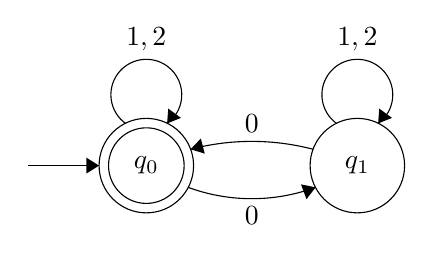
\begin{tikzpicture}[scale=0.2]
\tikzstyle{every node}+=[inner sep=0pt]
\draw [black] (12,-17.4) circle (3);
\draw (12,-17.4) node {$q_0$};
\draw [black] (12,-17.4) circle (2.4);
\draw [black] (25.4,-17.4) circle (3);
\draw (25.4,-17.4) node {$q_1$};
\draw [black] (4.5,-17.4) -- (9,-17.4);
\fill [black] (9,-17.4) -- (8.2,-16.9) -- (8.2,-17.9);
\draw [black] (22.746,-18.781) arc (-69.83394:-110.16606:11.736);
\fill [black] (22.75,-18.78) -- (21.82,-18.59) -- (22.17,-19.53);
\draw (18.7,-20) node [below] {$0$};
\draw [black] (14.81,-16.362) arc (104.68234:75.31766:15.349);
\fill [black] (14.81,-16.36) -- (15.71,-16.64) -- (15.46,-15.68);
\draw (18.7,-15.36) node [above] {$0$};
\draw [black] (10.677,-14.72) arc (234:-54:2.25);
\draw (12,-10.15) node [above] {$1,2$};
\fill [black] (13.32,-14.72) -- (14.2,-14.37) -- (13.39,-13.78);
\draw [black] (24.077,-14.72) arc (234:-54:2.25);
\draw (25.4,-10.15) node [above] {$1,2$};
\fill [black] (26.72,-14.72) -- (27.6,-14.37) -- (26.79,-13.78);
\end{tikzpicture}
\end{center}

Und dann bauen wir $M_2$:

\begin{center}
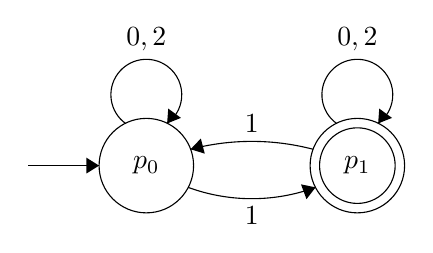
\begin{tikzpicture}[scale=0.2]
\tikzstyle{every node}+=[inner sep=0pt]
\draw [black] (12,-17.4) circle (3);
\draw (12,-17.4) node {$p_0$};
\draw [black] (25.4,-17.4) circle (3);
\draw (25.4,-17.4) node {$p_1$};
\draw [black] (25.4,-17.4) circle (2.4);
\draw [black] (4.5,-17.4) -- (9,-17.4);
\fill [black] (9,-17.4) -- (8.2,-16.9) -- (8.2,-17.9);
\draw [black] (22.746,-18.781) arc (-69.83394:-110.16606:11.736);
\fill [black] (22.75,-18.78) -- (21.82,-18.59) -- (22.17,-19.53);
\draw (18.7,-20) node [below] {$1$};
\draw [black] (14.81,-16.362) arc (104.68234:75.31766:15.349);
\fill [black] (14.81,-16.36) -- (15.71,-16.64) -- (15.46,-15.68);
\draw (18.7,-15.36) node [above] {$1$};
\draw [black] (10.677,-14.72) arc (234:-54:2.25);
\draw (12,-10.15) node [above] {$0,2$};
\fill [black] (13.32,-14.72) -- (14.2,-14.37) -- (13.39,-13.78);
\draw [black] (24.077,-14.72) arc (234:-54:2.25);
\draw (25.4,-10.15) node [above] {$0,2$};
\fill [black] (26.72,-14.72) -- (27.6,-14.37) -- (26.79,-13.78);
\end{tikzpicture}
\end{center}

Und schnurstracks $M_3$:

\begin{center}
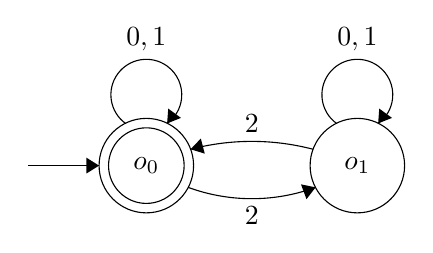
\begin{tikzpicture}[scale=0.2]
\tikzstyle{every node}+=[inner sep=0pt]
\draw [black] (12,-17.4) circle (3);
\draw (12,-17.4) node {$o_0$};
\draw [black] (12,-17.4) circle (2.4);
\draw [black] (25.4,-17.4) circle (3);
\draw (25.4,-17.4) node {$o_1$};
\draw [black] (4.5,-17.4) -- (9,-17.4);
\fill [black] (9,-17.4) -- (8.2,-16.9) -- (8.2,-17.9);
\draw [black] (22.746,-18.781) arc (-69.83394:-110.16606:11.736);
\fill [black] (22.75,-18.78) -- (21.82,-18.59) -- (22.17,-19.53);
\draw (18.7,-20) node [below] {$2$};
\draw [black] (14.81,-16.362) arc (104.68234:75.31766:15.349);
\fill [black] (14.81,-16.36) -- (15.71,-16.64) -- (15.46,-15.68);
\draw (18.7,-15.36) node [above] {$2$};
\draw [black] (10.677,-14.72) arc (234:-54:2.25);
\draw (12,-10.15) node [above] {$0,1$};
\fill [black] (13.32,-14.72) -- (14.2,-14.37) -- (13.39,-13.78);
\draw [black] (24.077,-14.72) arc (234:-54:2.25);
\draw (25.4,-10.15) node [above] {$0,1$};
\fill [black] (26.72,-14.72) -- (27.6,-14.37) -- (26.79,-13.78);
\end{tikzpicture}
\end{center}

Um die gewünschte Verknüpfung zu erreichen, bauen wir zunächst einen intermediären Automaten $M_{12}$, für den gilt $\mathcal{L}(M_{12}) = L_1 \cap L_2$ und darum $F_{M_{12}} = (F_{M_{1}} \times Q_{M_{2}}) \cap  (Q_{M_{1}} \times F_{M_{2}}) $:

\begin{center}
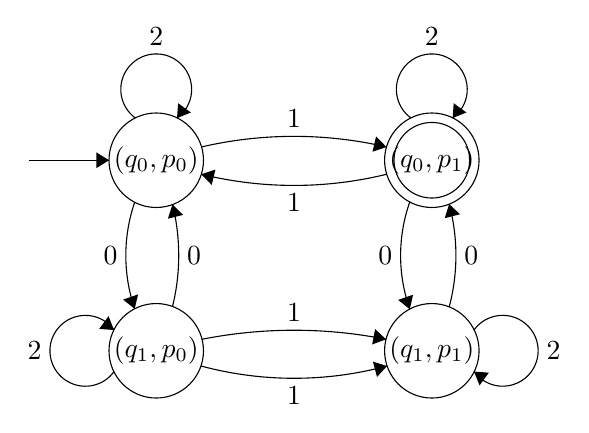
\begin{tikzpicture}[scale=0.2]
\tikzstyle{every node}+=[inner sep=0pt]
\draw [black] (18.2,-18.8) circle (3);
\draw (18.2,-18.8) node {$(q_0,p_0)$};
\draw [black] (35.7,-18.8) circle (3);
\draw (35.7,-18.8) node {$(q_0,p_1)$};
\draw [black] (35.7,-18.8) circle (2.4);
\draw [black] (18.2,-30.9) circle (3);
\draw (18.2,-30.9) node {$(q_1,p_0)$};
\draw [black] (35.7,-30.9) circle (3);
\draw (35.7,-30.9) node {$(q_1,p_1)$};
\draw [black] (10.1,-18.8) -- (15.2,-18.8);
\fill [black] (15.2,-18.8) -- (14.4,-18.3) -- (14.4,-19.3);
\draw [black] (16.834,-28.241) arc (-161.04272:-198.95728:10.437);
\fill [black] (16.83,-28.24) -- (17.05,-27.32) -- (16.1,-27.65);
\draw (15.77,-24.85) node [left] {$0$};
\draw [black] (21.077,-17.955) arc (103.06181:76.93819:25.987);
\fill [black] (32.82,-17.96) -- (32.16,-17.29) -- (31.93,-18.26);
\draw (26.95,-16.78) node [above] {$1$};
\draw [black] (16.877,-16.12) arc (234:-54:2.25);
\draw (18.2,-11.55) node [above] {$2$};
\fill [black] (19.52,-16.12) -- (20.4,-15.77) -- (19.59,-15.18);
\draw [black] (34.302,-28.258) arc (-160.52746:-199.47254:10.222);
\fill [black] (34.3,-28.26) -- (34.51,-27.34) -- (33.56,-27.67);
\draw (33.22,-24.85) node [left] {$0$};
\draw [black] (34.377,-16.12) arc (234:-54:2.25);
\draw (35.7,-11.55) node [above] {$2$};
\fill [black] (37.02,-16.12) -- (37.9,-15.77) -- (37.09,-15.18);
\draw [black] (15.52,-32.223) arc (324:36:2.25);
\draw (10.95,-30.9) node [left] {$2$};
\fill [black] (15.52,-29.58) -- (15.17,-28.7) -- (14.58,-29.51);
\draw [black] (38.38,-29.577) arc (144:-144:2.25);
\draw (42.95,-30.9) node [right] {$2$};
\fill [black] (38.38,-32.22) -- (38.73,-33.1) -- (39.32,-32.29);
\draw [black] (32.837,-19.689) arc (-76.22291:-103.77709:24.719);
\fill [black] (21.06,-19.69) -- (21.72,-20.37) -- (21.96,-19.39);
\draw (26.95,-20.9) node [below] {$1$};
\draw [black] (21.108,-30.169) arc (101.23374:78.76626:29.986);
\fill [black] (32.79,-30.17) -- (32.1,-29.52) -- (31.91,-30.5);
\draw (26.95,-29.09) node [above] {$1$};
\draw [black] (32.862,-31.866) arc (-74.96866:-105.03134:22.796);
\fill [black] (32.86,-31.87) -- (31.96,-31.59) -- (32.22,-32.56);
\draw (26.95,-33.15) node [below] {$1$};
\draw [black] (19.234,-21.61) arc (13.85337:-13.85337:13.533);
\fill [black] (19.23,-21.61) -- (18.94,-22.51) -- (19.91,-22.27);
\draw (20.13,-24.85) node [right] {$0$};
\draw [black] (36.803,-21.582) arc (14.87178:-14.87178:12.731);
\fill [black] (36.8,-21.58) -- (36.52,-22.48) -- (37.49,-22.23);
\draw (37.73,-24.85) node [right] {$0$};
\end{tikzpicture}
\end{center}

Nun benennen wir die Zustände um, weil die Kreise zu klein werden:
\begin{tabular}{rcl}
$(q_0,p_0)$ & $\mapsto$ & $A$ \\
$(q_0,p_1)$ & $\mapsto$ & $B$ \\
$(q_1,p_0)$ & $\mapsto$ & $C$ \\
$(q_1,p_1)$ & $\mapsto$ & $D$ \\
\end{tabular}

\begin{center}
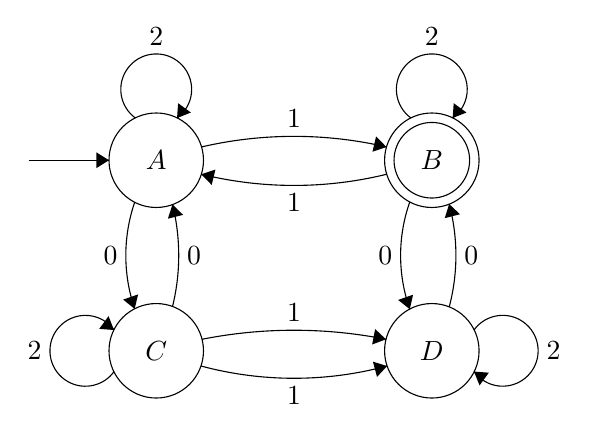
\begin{tikzpicture}[scale=0.2]
\tikzstyle{every node}+=[inner sep=0pt]
\draw [black] (18.2,-18.8) circle (3);
\draw (18.2,-18.8) node {$A$};
\draw [black] (35.7,-18.8) circle (3);
\draw (35.7,-18.8) node {$B$};
\draw [black] (35.7,-18.8) circle (2.4);
\draw [black] (18.2,-30.9) circle (3);
\draw (18.2,-30.9) node {$C$};
\draw [black] (35.7,-30.9) circle (3);
\draw (35.7,-30.9) node {$D$};
\draw [black] (10.1,-18.8) -- (15.2,-18.8);
\fill [black] (15.2,-18.8) -- (14.4,-18.3) -- (14.4,-19.3);
\draw [black] (16.834,-28.241) arc (-161.04272:-198.95728:10.437);
\fill [black] (16.83,-28.24) -- (17.05,-27.32) -- (16.1,-27.65);
\draw (15.77,-24.85) node [left] {$0$};
\draw [black] (21.077,-17.955) arc (103.06181:76.93819:25.987);
\fill [black] (32.82,-17.96) -- (32.16,-17.29) -- (31.93,-18.26);
\draw (26.95,-16.78) node [above] {$1$};
\draw [black] (16.877,-16.12) arc (234:-54:2.25);
\draw (18.2,-11.55) node [above] {$2$};
\fill [black] (19.52,-16.12) -- (20.4,-15.77) -- (19.59,-15.18);
\draw [black] (34.302,-28.258) arc (-160.52746:-199.47254:10.222);
\fill [black] (34.3,-28.26) -- (34.51,-27.34) -- (33.56,-27.67);
\draw (33.22,-24.85) node [left] {$0$};
\draw [black] (34.377,-16.12) arc (234:-54:2.25);
\draw (35.7,-11.55) node [above] {$2$};
\fill [black] (37.02,-16.12) -- (37.9,-15.77) -- (37.09,-15.18);
\draw [black] (15.52,-32.223) arc (324:36:2.25);
\draw (10.95,-30.9) node [left] {$2$};
\fill [black] (15.52,-29.58) -- (15.17,-28.7) -- (14.58,-29.51);
\draw [black] (38.38,-29.577) arc (144:-144:2.25);
\draw (42.95,-30.9) node [right] {$2$};
\fill [black] (38.38,-32.22) -- (38.73,-33.1) -- (39.32,-32.29);
\draw [black] (32.837,-19.689) arc (-76.22291:-103.77709:24.719);
\fill [black] (21.06,-19.69) -- (21.72,-20.37) -- (21.96,-19.39);
\draw (26.95,-20.9) node [below] {$1$};
\draw [black] (21.108,-30.169) arc (101.23374:78.76626:29.986);
\fill [black] (32.79,-30.17) -- (32.1,-29.52) -- (31.91,-30.5);
\draw (26.95,-29.09) node [above] {$1$};
\draw [black] (32.862,-31.866) arc (-74.96866:-105.03134:22.796);
\fill [black] (32.86,-31.87) -- (31.96,-31.59) -- (32.22,-32.56);
\draw (26.95,-33.15) node [below] {$1$};
\draw [black] (19.234,-21.61) arc (13.85337:-13.85337:13.533);
\fill [black] (19.23,-21.61) -- (18.94,-22.51) -- (19.91,-22.27);
\draw (20.13,-24.85) node [right] {$0$};
\draw [black] (36.803,-21.582) arc (14.87178:-14.87178:12.731);
\fill [black] (36.8,-21.58) -- (36.52,-22.48) -- (37.49,-22.23);
\draw (37.73,-24.85) node [right] {$0$};
\end{tikzpicture}
\end{center}

Und verknüpfen nach dem bekannten Schema $M_{12}$ und $M_3$ zu $M$, so dass $\mathcal{L}(M) = \mathcal{L}(M_{12}) \cup \mathcal{L}(M_3):$

\begin{center}
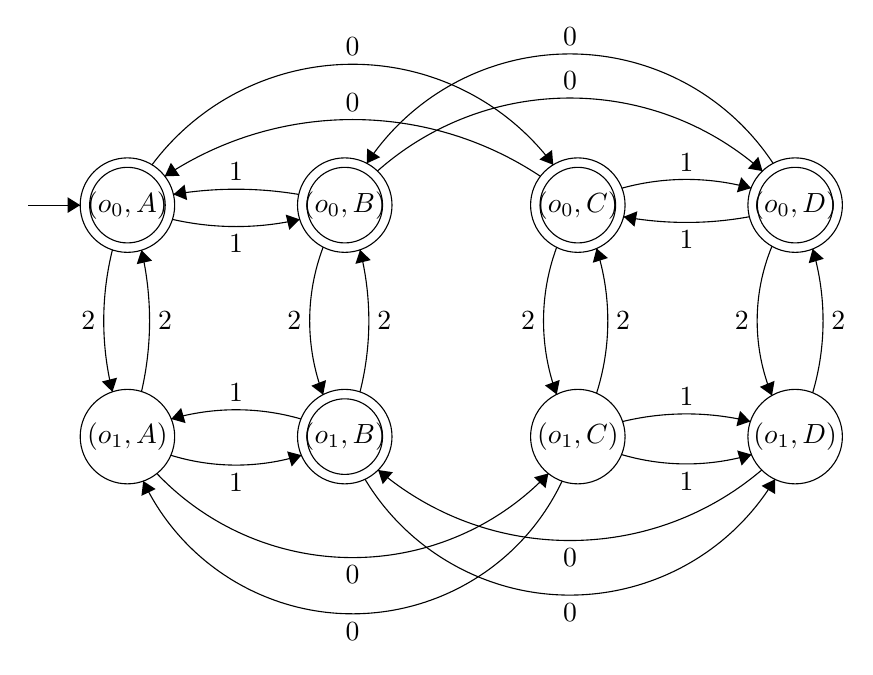
\begin{tikzpicture}[scale=0.2]
\tikzstyle{every node}+=[inner sep=0pt]
\draw [black] (10.8,-18) circle (3);
\draw (10.8,-18) node {$(o_0,A)$};
\draw [black] (10.8,-18) circle (2.4);
\draw [black] (24.6,-18) circle (3);
\draw (24.6,-18) node {$(o_0,B)$};
\draw [black] (24.6,-18) circle (2.4);
\draw [black] (39.4,-18) circle (3);
\draw (39.4,-18) node {$(o_0,C)$};
\draw [black] (39.4,-18) circle (2.4);
\draw [black] (53.2,-18) circle (3);
\draw (53.2,-18) node {$(o_0,D)$};
\draw [black] (53.2,-18) circle (2.4);
\draw [black] (10.8,-32.7) circle (3);
\draw (10.8,-32.7) node {$(o_1,A)$};
\draw [black] (24.6,-32.7) circle (3);
\draw (24.6,-32.7) node {$(o_1,B)$};
\draw [black] (24.6,-32.7) circle (2.4);
\draw [black] (53.2,-32.7) circle (3);
\draw (53.2,-32.7) node {$(o_1,D)$};
\draw [black] (39.4,-32.7) circle (3);
\draw (39.4,-32.7) node {$(o_1,C)$};
\draw [black] (4.5,-18) -- (7.8,-18);
\fill [black] (7.8,-18) -- (7,-17.5) -- (7,-18.5);
\draw [black] (12.359,-15.442) arc (143.24479:36.75521:15.903);
\fill [black] (37.84,-15.44) -- (37.76,-14.5) -- (36.96,-15.1);
\draw (25.1,-8.56) node [above] {$0$};
\draw [black] (21.744,-18.906) arc (-77.13283:-102.86717:18.158);
\fill [black] (21.74,-18.91) -- (20.85,-18.6) -- (21.08,-19.57);
\draw (17.7,-19.86) node [below] {$1$};
\draw [black] (9.846,-29.859) arc (-166.04379:-193.95621:18.695);
\fill [black] (9.85,-29.86) -- (10.14,-28.96) -- (9.17,-29.2);
\draw (8.79,-25.35) node [left] {$2$};
\draw [black] (26.674,-15.837) arc (131.54717:48.45283:18.434);
\fill [black] (51.13,-15.84) -- (50.86,-14.93) -- (50.2,-15.68);
\draw (38.9,-10.7) node [above] {$0$};
\draw [black] (13.72,-17.321) arc (99.51711:80.48289:24.07);
\fill [black] (13.72,-17.32) -- (14.59,-17.68) -- (14.43,-16.7);
\draw (17.7,-16.49) node [above] {$1$};
\draw [black] (23.23,-30.038) arc (-159.26416:-200.73584:13.241);
\fill [black] (23.23,-30.04) -- (23.41,-29.11) -- (22.48,-29.47);
\draw (21.87,-25.35) node [left] {$2$};
\draw [black] (13.174,-16.17) arc (123.62919:56.37081:21.534);
\fill [black] (13.17,-16.17) -- (14.12,-16.14) -- (13.56,-15.31);
\draw (25.1,-12.07) node [above] {$0$};
\draw [black] (42.196,-16.925) arc (105.45938:74.54062:15.398);
\fill [black] (50.4,-16.92) -- (49.77,-16.23) -- (49.5,-17.19);
\draw (46.3,-15.87) node [above] {$1$};
\draw [black] (38.057,-30.024) arc (-159.72766:-200.27234:13.49);
\fill [black] (38.06,-30.02) -- (38.25,-29.1) -- (37.31,-29.45);
\draw (36.72,-25.35) node [left] {$2$};
\draw [black] (25.997,-15.351) arc (146.63075:33.36925:15.45);
\fill [black] (26,-15.35) -- (26.85,-14.96) -- (26.02,-14.41);
\draw (38.9,-7.9) node [above] {$0$};
\draw [black] (50.294,-18.738) arc (-79.63007:-100.36993:22.191);
\fill [black] (42.31,-18.74) -- (43,-19.37) -- (43.18,-18.39);
\draw (46.3,-19.6) node [below] {$1$};
\draw [black] (51.73,-30.093) arc (-157.51888:-202.48112:12.404);
\fill [black] (51.73,-30.09) -- (51.89,-29.16) -- (50.96,-29.54);
\draw (50.29,-25.35) node [left] {$2$};
\draw [black] (11.693,-20.861) arc (13.02549:-13.02549:19.917);
\fill [black] (11.69,-20.86) -- (11.39,-21.75) -- (12.36,-21.53);
\draw (12.71,-25.35) node [right] {$2$};
\draw [black] (25.568,-20.836) arc (14.18558:-14.18558:18.42);
\fill [black] (25.57,-20.84) -- (25.28,-21.73) -- (26.25,-21.49);
\draw (26.63,-25.35) node [right] {$2$};
\draw [black] (40.588,-20.749) arc (17.69236:-17.69236:15.138);
\fill [black] (40.59,-20.75) -- (40.35,-21.66) -- (41.31,-21.36);
\draw (41.8,-25.35) node [right] {$2$};
\draw [black] (54.312,-20.782) arc (16.45373:-16.45373:16.128);
\fill [black] (54.31,-20.78) -- (54.06,-21.69) -- (55.02,-21.41);
\draw (55.47,-25.35) node [right] {$2$};
\draw [black] (21.849,-33.883) arc (-72.84146:-107.15854:14.064);
\fill [black] (21.85,-33.88) -- (20.94,-33.64) -- (21.23,-34.6);
\draw (17.7,-35.01) node [below] {$1$};
\draw [black] (13.578,-31.58) arc (106.1608:73.8392:14.811);
\fill [black] (13.58,-31.58) -- (14.49,-31.84) -- (14.21,-30.88);
\draw (17.7,-30.49) node [above] {$1$};
\draw [black] (50.43,-33.838) arc (-73.5608:-106.4392:14.593);
\fill [black] (50.43,-33.84) -- (49.52,-33.58) -- (49.8,-34.54);
\draw (46.3,-34.93) node [below] {$1$};
\draw [black] (42.239,-31.743) arc (103.63018:76.36982:17.231);
\fill [black] (50.36,-31.74) -- (49.7,-31.07) -- (49.47,-32.04);
\draw (46.3,-30.76) node [above] {$1$};
\draw [black] (37.534,-35.044) arc (-43.52594:-136.47406:17.149);
\fill [black] (37.53,-35.04) -- (36.62,-35.28) -- (37.35,-35.97);
\draw (25.1,-40.88) node [below] {$0$};
\draw [black] (38.402,-35.524) arc (-25.29782:-154.70218:14.713);
\fill [black] (11.8,-35.52) -- (11.69,-36.46) -- (12.59,-36.03);
\draw (25.1,-44.45) node [below] {$0$};
\draw [black] (51.916,-35.406) arc (-31.04705:-148.95295:15.192);
\fill [black] (51.92,-35.41) -- (51.07,-35.83) -- (51.93,-36.35);
\draw (38.9,-43.26) node [below] {$0$};
\draw [black] (51.08,-34.818) arc (-49.6052:-130.3948:18.794);
\fill [black] (26.72,-34.82) -- (27.01,-35.72) -- (27.65,-34.96);
\draw (38.9,-39.8) node [below] {$0$};
\end{tikzpicture}
\end{center}

\section*{Kontrollaufgabe 2(f)}

Bauen wir noch ein paar Automaten mehr. $M_1$ akzeptiere $L_1$:

\begin{center}
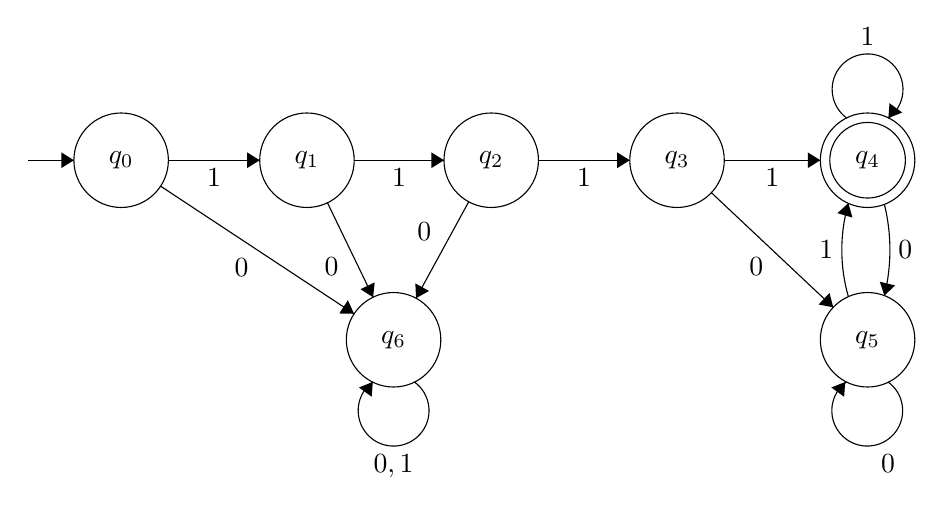
\begin{tikzpicture}[scale=0.2]
\tikzstyle{every node}+=[inner sep=0pt]
\draw [black] (10.3,-15.5) circle (3);
\draw (10.3,-15.5) node {$q_0$};
\draw [black] (22.1,-15.5) circle (3);
\draw (22.1,-15.5) node {$q_1$};
\draw [black] (33.8,-15.5) circle (3);
\draw (33.8,-15.5) node {$q_2$};
\draw [black] (45.6,-15.5) circle (3);
\draw (45.6,-15.5) node {$q_3$};
\draw [black] (57.7,-15.5) circle (3);
\draw (57.7,-15.5) node {$q_4$};
\draw [black] (57.7,-15.5) circle (2.4);
\draw [black] (57.7,-26.9) circle (3);
\draw (57.7,-26.9) node {$q_5$};
\draw [black] (27.6,-26.9) circle (3);
\draw (27.6,-26.9) node {$q_6$};
\draw [black] (4.4,-15.5) -- (7.3,-15.5);
\fill [black] (7.3,-15.5) -- (6.5,-15) -- (6.5,-16);
\draw [black] (13.3,-15.5) -- (19.1,-15.5);
\fill [black] (19.1,-15.5) -- (18.3,-15) -- (18.3,-16);
\draw (16.2,-16) node [below] {$1$};
\draw [black] (25.1,-15.5) -- (30.8,-15.5);
\fill [black] (30.8,-15.5) -- (30,-15) -- (30,-16);
\draw (27.95,-16) node [below] {$1$};
\draw [black] (36.8,-15.5) -- (42.6,-15.5);
\fill [black] (42.6,-15.5) -- (41.8,-15) -- (41.8,-16);
\draw (39.7,-16) node [below] {$1$};
\draw [black] (56.377,-12.82) arc (234:-54:2.25);
\draw (57.7,-8.25) node [above] {$1$};
\fill [black] (59.02,-12.82) -- (59.9,-12.47) -- (59.09,-11.88);
\draw [black] (48.6,-15.5) -- (54.7,-15.5);
\fill [black] (54.7,-15.5) -- (53.9,-15) -- (53.9,-16);
\draw (51.65,-16) node [below] {$1$};
\draw [black] (47.78,-17.56) -- (55.52,-24.84);
\fill [black] (55.52,-24.84) -- (55.28,-23.93) -- (54.59,-24.66);
\draw (50.63,-21.68) node [below] {$0$};
\draw [black] (56.481,-24.169) arc (-163.94954:-196.05046:10.74);
\fill [black] (56.48,-18.23) -- (55.78,-18.86) -- (56.74,-19.14);
\draw (55.56,-21.2) node [left] {$1$};
\draw [black] (58.766,-18.296) arc (13.80507:-13.80507:12.169);
\fill [black] (58.77,-24.1) -- (59.44,-23.45) -- (58.47,-23.21);
\draw (59.62,-21.2) node [right] {$0$};
\draw [black] (28.923,-29.58) arc (54:-234:2.25);
\draw (27.6,-34.15) node [below] {$0,1$};
\fill [black] (26.28,-29.58) -- (25.4,-29.93) -- (26.21,-30.52);
\draw [black] (12.81,-17.15) -- (25.09,-25.25);
\fill [black] (25.09,-25.25) -- (24.7,-24.39) -- (24.15,-25.23);
\draw (17.95,-21.7) node [below] {$0$};
\draw [black] (23.4,-18.2) -- (26.3,-24.2);
\fill [black] (26.3,-24.2) -- (26.4,-23.26) -- (25.5,-23.69);
\draw (24.14,-22.27) node [left] {$0$};
\draw [black] (32.37,-18.14) -- (29.03,-24.26);
\fill [black] (29.03,-24.26) -- (29.85,-23.8) -- (28.98,-23.32);
\draw (30.03,-20.02) node [left] {$0$};

\draw [black] (59,-29.58) arc (54:-234:2.25);
\draw (59,-34.15) node [below] {$0$};
\fill [black] (56.28,-29.58) -- (55.4,-29.93) -- (56.21,-30.52);

\end{tikzpicture}
\end{center}

$M_1^C$ akzeptiere $\{0,1\}^* - L_1$ (durch $F_{M_1^C} = Q_{M_1} - F_{M_1}$). Man könnte auch diesen Automaten durch modulare Konstruktion bauen, es wäre die Verknüpfung des "neutralen" Automaten $(\{p_0\}, \{0,1\}, p_0, \delta(p) = p, \{p_0\})$ mit $M_1$, wobei die akzeptierenden Zustände $F_{M_1^C} = \{p_0\} \times (Q_{M_1} - F_{M_1})$ wären. Bringt ausser mehr Schreibarbeit nichts, darum lasse ich das bleiben. Hier darum direkt $M_1^C$:

\begin{center}
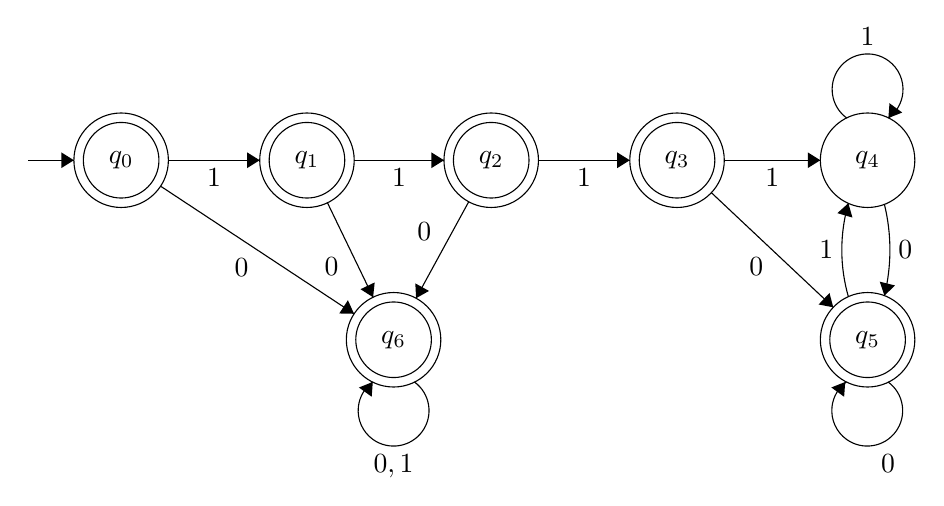
\begin{tikzpicture}[scale=0.2]
\tikzstyle{every node}+=[inner sep=0pt]
\draw [black] (10.3,-15.5) circle (3);
\draw (10.3,-15.5) node {$q_0$};
\draw [black] (10.3,-15.5) circle (2.4);
\draw [black] (22.1,-15.5) circle (3);
\draw (22.1,-15.5) node {$q_1$};
\draw [black] (22.1,-15.5) circle (2.4);
\draw [black] (33.8,-15.5) circle (3);
\draw (33.8,-15.5) node {$q_2$};
\draw [black] (33.8,-15.5) circle (2.4);
\draw [black] (45.6,-15.5) circle (3);
\draw (45.6,-15.5) node {$q_3$};
\draw [black] (45.6,-15.5) circle (2.4);
\draw [black] (57.7,-15.5) circle (3);
\draw (57.7,-15.5) node {$q_4$};
\draw [black] (57.7,-26.9) circle (3);
\draw (57.7,-26.9) node {$q_5$};
\draw [black] (57.7,-26.9) circle (2.4);
\draw [black] (27.6,-26.9) circle (3);
\draw (27.6,-26.9) node {$q_6$};
\draw [black] (27.6,-26.9) circle (2.4);
\draw [black] (4.4,-15.5) -- (7.3,-15.5);
\fill [black] (7.3,-15.5) -- (6.5,-15) -- (6.5,-16);
\draw [black] (13.3,-15.5) -- (19.1,-15.5);
\fill [black] (19.1,-15.5) -- (18.3,-15) -- (18.3,-16);
\draw (16.2,-16) node [below] {$1$};
\draw [black] (25.1,-15.5) -- (30.8,-15.5);
\fill [black] (30.8,-15.5) -- (30,-15) -- (30,-16);
\draw (27.95,-16) node [below] {$1$};
\draw [black] (36.8,-15.5) -- (42.6,-15.5);
\fill [black] (42.6,-15.5) -- (41.8,-15) -- (41.8,-16);
\draw (39.7,-16) node [below] {$1$};
\draw [black] (56.377,-12.82) arc (234:-54:2.25);
\draw (57.7,-8.25) node [above] {$1$};
\fill [black] (59.02,-12.82) -- (59.9,-12.47) -- (59.09,-11.88);
\draw [black] (48.6,-15.5) -- (54.7,-15.5);
\fill [black] (54.7,-15.5) -- (53.9,-15) -- (53.9,-16);
\draw (51.65,-16) node [below] {$1$};
\draw [black] (47.78,-17.56) -- (55.52,-24.84);
\fill [black] (55.52,-24.84) -- (55.28,-23.93) -- (54.59,-24.66);
\draw (50.63,-21.68) node [below] {$0$};
\draw [black] (56.481,-24.169) arc (-163.94954:-196.05046:10.74);
\fill [black] (56.48,-18.23) -- (55.78,-18.86) -- (56.74,-19.14);
\draw (55.56,-21.2) node [left] {$1$};
\draw [black] (58.766,-18.296) arc (13.80507:-13.80507:12.169);
\fill [black] (58.77,-24.1) -- (59.44,-23.45) -- (58.47,-23.21);
\draw (59.62,-21.2) node [right] {$0$};
\draw [black] (28.923,-29.58) arc (54:-234:2.25);
\draw (27.6,-34.15) node [below] {$0,1$};
\fill [black] (26.28,-29.58) -- (25.4,-29.93) -- (26.21,-30.52);
\draw [black] (12.81,-17.15) -- (25.09,-25.25);
\fill [black] (25.09,-25.25) -- (24.7,-24.39) -- (24.15,-25.23);
\draw (17.95,-21.7) node [below] {$0$};
\draw [black] (23.4,-18.2) -- (26.3,-24.2);
\fill [black] (26.3,-24.2) -- (26.4,-23.26) -- (25.5,-23.69);
\draw (24.14,-22.27) node [left] {$0$};
\draw [black] (32.37,-18.14) -- (29.03,-24.26);
\fill [black] (29.03,-24.26) -- (29.85,-23.8) -- (28.98,-23.32);
\draw (30.03,-20.02) node [left] {$0$};

\draw [black] (59,-29.58) arc (54:-234:2.25);
\draw (59,-34.15) node [below] {$0$};
\fill [black] (56.28,-29.58) -- (55.4,-29.93) -- (56.21,-30.52);

\end{tikzpicture}
\end{center}

$M_3$ (mit $\mathcal{L}(M_3) = L_3$) brauchts natürlich auch:

\begin{center}
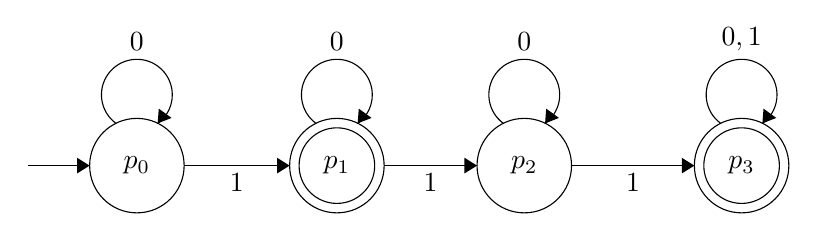
\begin{tikzpicture}[scale=0.2]
\tikzstyle{every node}+=[inner sep=0pt]
\draw [black] (14.6,-20.5) circle (3);
\draw (14.6,-20.5) node {$p_0$};
\draw [black] (27.3,-20.5) circle (3);
\draw (27.3,-20.5) node {$p_1$};
\draw [black] (27.3,-20.5) circle (2.4);
\draw [black] (39.2,-20.5) circle (3);
\draw (39.2,-20.5) node {$p_2$};
\draw [black] (53,-20.5) circle (3);
\draw (53,-20.5) node {$p_3$};
\draw [black] (53,-20.5) circle (2.4);
\draw [black] (7.7,-20.5) -- (11.6,-20.5);
\fill [black] (11.6,-20.5) -- (10.8,-20) -- (10.8,-21);
\draw [black] (17.6,-20.5) -- (24.3,-20.5);
\fill [black] (24.3,-20.5) -- (23.5,-20) -- (23.5,-21);
\draw (20.95,-21) node [below] {$1$};
\draw [black] (13.277,-17.82) arc (234:-54:2.25);
\draw (14.6,-13.25) node [above] {$0$};
\fill [black] (15.92,-17.82) -- (16.8,-17.47) -- (15.99,-16.88);
\draw [black] (30.3,-20.5) -- (36.2,-20.5);
\fill [black] (36.2,-20.5) -- (35.4,-20) -- (35.4,-21);
\draw (33.25,-21) node [below] {$1$};
\draw [black] (25.977,-17.82) arc (234:-54:2.25);
\draw (27.3,-13.25) node [above] {$0$};
\fill [black] (28.62,-17.82) -- (29.5,-17.47) -- (28.69,-16.88);
\draw [black] (37.877,-17.82) arc (234:-54:2.25);
\draw (39.2,-13.25) node [above] {$0$};
\fill [black] (40.52,-17.82) -- (41.4,-17.47) -- (40.59,-16.88);
\draw [black] (42.2,-20.5) -- (50,-20.5);
\fill [black] (50,-20.5) -- (49.2,-20) -- (49.2,-21);
\draw (46.1,-21) node [below] {$1$};
\draw [black] (51.677,-17.82) arc (234:-54:2.25);
\draw (53,-13.25) node [above] {$0,1$};
\fill [black] (54.32,-17.82) -- (55.2,-17.47) -- (54.39,-16.88);
\end{tikzpicture}
\end{center}

Was bei der Konstruktion des finalen Automaten zu einer Matrix mit 28 (neuer Rekord!) Zuständen führt:

\begin{center}
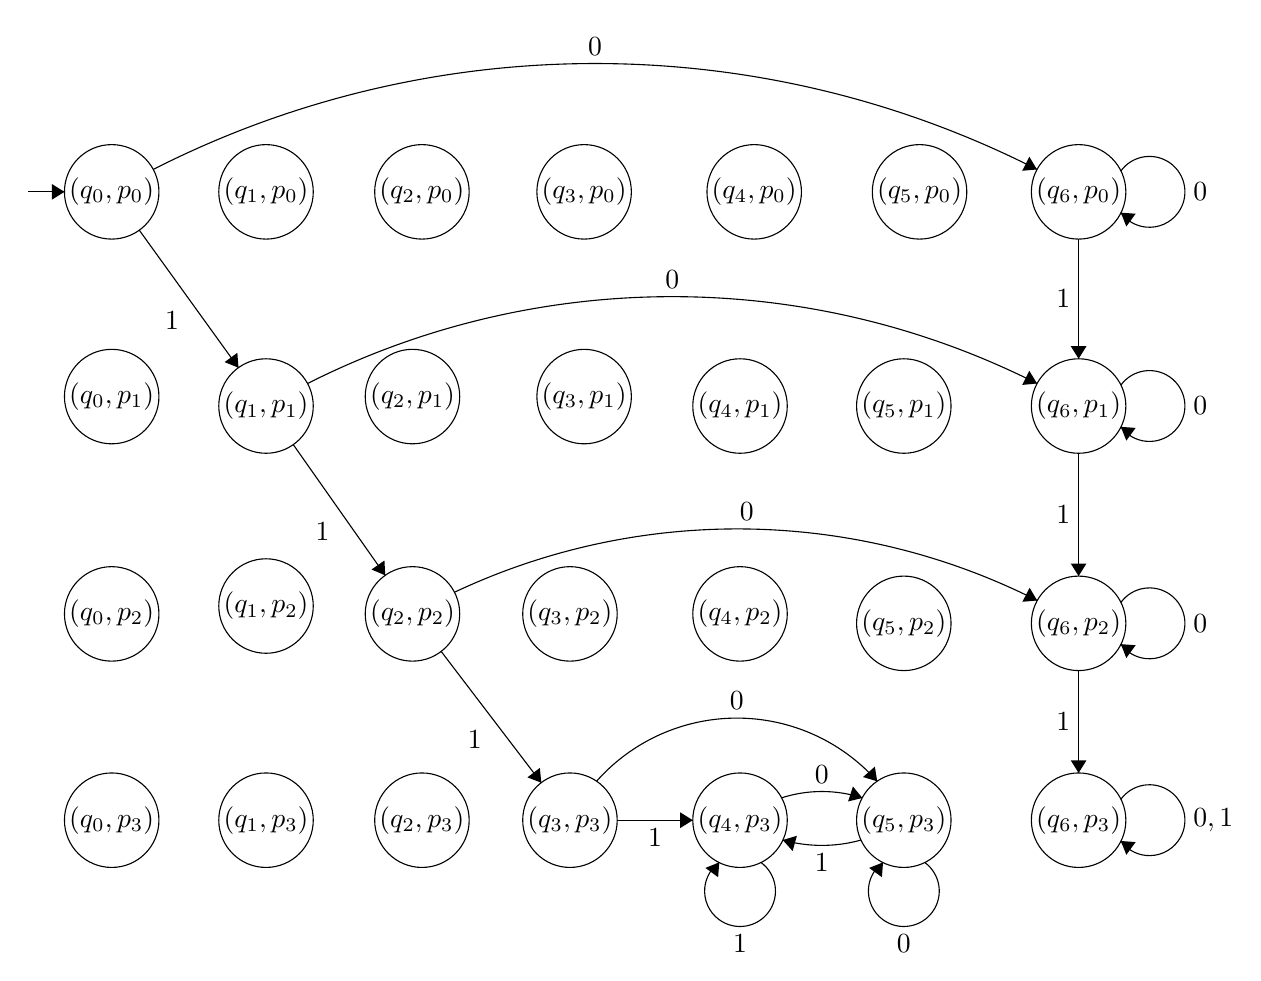
\begin{tikzpicture}[scale=0.2]
\tikzstyle{every node}+=[inner sep=0pt]
\draw [black] (7.8,-11) circle (3);
\draw (7.8,-11) node {$(q_0,p_0)$};
\draw [black] (17.6,-11) circle (3);
\draw (17.6,-11) node {$(q_1,p_0)$};
\draw [black] (27.5,-11) circle (3);
\draw (27.5,-11) node {$(q_2,p_0)$};
\draw [black] (37.8,-11) circle (3);
\draw (37.8,-11) node {$(q_3,p_0)$};
\draw [black] (48.6,-11) circle (3);
\draw (48.6,-11) node {$(q_4,p_0)$};
\draw [black] (59.1,-11) circle (3);
\draw (59.1,-11) node {$(q_5,p_0)$};
\draw [black] (69.2,-11) circle (3);
\draw (69.2,-11) node {$(q_6,p_0)$};
\draw [black] (7.8,-24) circle (3);
\draw (7.8,-24) node {$(q_0,p_1)$};
\draw [black] (17.6,-24.6) circle (3);
\draw (17.6,-24.6) node {$(q_1,p_1)$};
\draw [black] (26.9,-24) circle (3);
\draw (26.9,-24) node {$(q_2,p_1)$};
\draw [black] (37.8,-24) circle (3);
\draw (37.8,-24) node {$(q_3,p_1)$};
\draw [black] (47.7,-24.6) circle (3);
\draw (47.7,-24.6) node {$(q_4,p_1)$};
\draw [black] (58.1,-24.6) circle (3);
\draw (58.1,-24.6) node {$(q_5,p_1)$};
\draw [black] (69.2,-24.6) circle (3);
\draw (69.2,-24.6) node {$(q_6,p_1)$};
\draw [black] (7.8,-37.8) circle (3);
\draw (7.8,-37.8) node {$(q_0,p_2)$};
\draw [black] (26.9,-37.8) circle (3);
\draw (26.9,-37.8) node {$(q_2,p_2)$};
\draw [black] (36.9,-37.8) circle (3);
\draw (36.9,-37.8) node {$(q_3,p_2)$};
\draw [black] (47.7,-37.8) circle (3);
\draw (47.7,-37.8) node {$(q_4,p_2)$};
\draw [black] (58.1,-38.4) circle (3);
\draw (58.1,-38.4) node {$(q_5,p_2)$};
\draw [black] (69.2,-38.4) circle (3);
\draw (69.2,-38.4) node {$(q_6,p_2)$};
\draw [black] (7.8,-50.9) circle (3);
\draw (7.8,-50.9) node {$(q_0,p_3)$};
\draw [black] (17.6,-50.9) circle (3);
\draw (17.6,-50.9) node {$(q_1,p_3)$};
\draw [black] (27.5,-50.9) circle (3);
\draw (27.5,-50.9) node {$(q_2,p_3)$};
\draw [black] (36.9,-50.9) circle (3);
\draw (36.9,-50.9) node {$(q_3,p_3)$};
\draw [black] (47.7,-50.9) circle (3);
\draw (47.7,-50.9) node {$(q_4,p_3)$};
\draw [black] (58.1,-50.9) circle (3);
\draw (58.1,-50.9) node {$(q_5,p_3)$};
\draw [black] (69.2,-50.9) circle (3);
\draw (69.2,-50.9) node {$(q_6,p_3)$};
\draw [black] (17.6,-37.3) circle (3);
\draw (17.6,-37.3) node {$(q_1,p_2)$};
\draw [black] (2.5,-11) -- (4.8,-11);
\fill [black] (4.8,-11) -- (4,-10.5) -- (4,-11.5);
\draw [black] (10.44,-9.576) arc (116.96031:63.03969:61.892);
\fill [black] (66.56,-9.58) -- (66.07,-8.77) -- (65.62,-9.66);
\draw (38.5,-2.35) node [above] {$0$};
\draw [black] (9.55,-13.43) -- (15.85,-22.17);
\fill [black] (15.85,-22.17) -- (15.78,-21.22) -- (14.97,-21.81);
\draw (12.11,-19.18) node [left] {$1$};
\draw [black] (71.88,-9.677) arc (144:-144:2.25);
\draw (76.45,-11) node [right] {$0$};
\fill [black] (71.88,-12.32) -- (72.23,-13.2) -- (72.82,-12.39);
\draw [black] (69.2,-14) -- (69.2,-21.6);
\fill [black] (69.2,-21.6) -- (69.7,-20.8) -- (68.7,-20.8);
\draw (68.7,-17.8) node [left] {$1$};
\draw [black] (20.237,-23.17) arc (116.79564:63.20436:51.381);
\fill [black] (66.56,-23.17) -- (66.07,-22.36) -- (65.62,-23.26);
\draw (43.4,-17.15) node [above] {$0$};
\draw [black] (19.33,-27.05) -- (25.17,-35.35);
\fill [black] (25.17,-35.35) -- (25.12,-34.41) -- (24.3,-34.98);
\draw (21.66,-32.57) node [left] {$1$};
\draw [black] (71.88,-23.277) arc (144:-144:2.25);
\draw (76.45,-24.6) node [right] {$0$};
\fill [black] (71.88,-25.92) -- (72.23,-26.8) -- (72.82,-25.99);
\draw [black] (69.2,-27.6) -- (69.2,-35.4);
\fill [black] (69.2,-35.4) -- (69.7,-34.6) -- (68.7,-34.6);
\draw (68.7,-31.5) node [left] {$1$};
\draw [black] (29.566,-36.425) arc (115.23657:63.13813:42.141);
\fill [black] (66.57,-36.95) -- (66.09,-36.14) -- (65.63,-37.03);
\draw (48.13,-31.89) node [above] {$0$};
\draw [black] (28.72,-40.18) -- (35.08,-48.52);
\fill [black] (35.08,-48.52) -- (34.99,-47.58) -- (34.2,-48.18);
\draw (31.33,-45.75) node [left] {$1$};
\draw [black] (71.88,-37.077) arc (144:-144:2.25);
\draw (76.45,-38.4) node [right] {$0$};
\fill [black] (71.88,-39.72) -- (72.23,-40.6) -- (72.82,-39.79);
\draw [black] (69.2,-41.4) -- (69.2,-47.9);
\fill [black] (69.2,-47.9) -- (69.7,-47.1) -- (68.7,-47.1);
\draw (68.7,-44.65) node [left] {$1$};
\draw [black] (38.587,-48.429) arc (138.47257:41.52743:11.906);
\fill [black] (56.41,-48.43) -- (56.26,-47.5) -- (55.51,-48.16);
\draw (47.5,-43.92) node [above] {$0$};
\draw [black] (39.9,-50.9) -- (44.7,-50.9);
\fill [black] (44.7,-50.9) -- (43.9,-50.4) -- (43.9,-51.4);
\draw (42.3,-51.4) node [below] {$1$};
\draw [black] (49.023,-53.58) arc (54:-234:2.25);
\draw (47.7,-58.15) node [below] {$1$};
\fill [black] (46.38,-53.58) -- (45.5,-53.93) -- (46.31,-54.52);
\draw [black] (50.327,-49.485) arc (107.98413:72.01587:8.333);
\fill [black] (55.47,-49.49) -- (54.87,-48.76) -- (54.56,-49.71);
\draw (52.9,-48.58) node [above] {$0$};
\draw [black] (55.391,-52.159) arc (-74.37127:-105.62873:9.247);
\fill [black] (50.41,-52.16) -- (51.04,-52.86) -- (51.31,-51.89);
\draw (52.9,-53) node [below] {$1$};
\draw [black] (59.423,-53.58) arc (54:-234:2.25);
\draw (58.1,-58.15) node [below] {$0$};
\fill [black] (56.78,-53.58) -- (55.9,-53.93) -- (56.71,-54.52);
\draw [black] (71.88,-49.577) arc (144:-144:2.25);
\draw (76.45,-50.9) node [right] {$0,1$};
\fill [black] (71.88,-52.22) -- (72.23,-53.1) -- (72.82,-52.29);
\end{tikzpicture}
\end{center}

Entfernen wir alles Unerreichbare, und überlegen wir uns die akzeptierenden Zustände:

\[
\mathcal{L}(M) = \mathcal{L}(M_3) - \mathcal{L}(M_1^C)
\Rightarrow F_M = F_{M_3} \times (Q_{M_1^C} - F_{M_1^C})
\]

\begin{center}
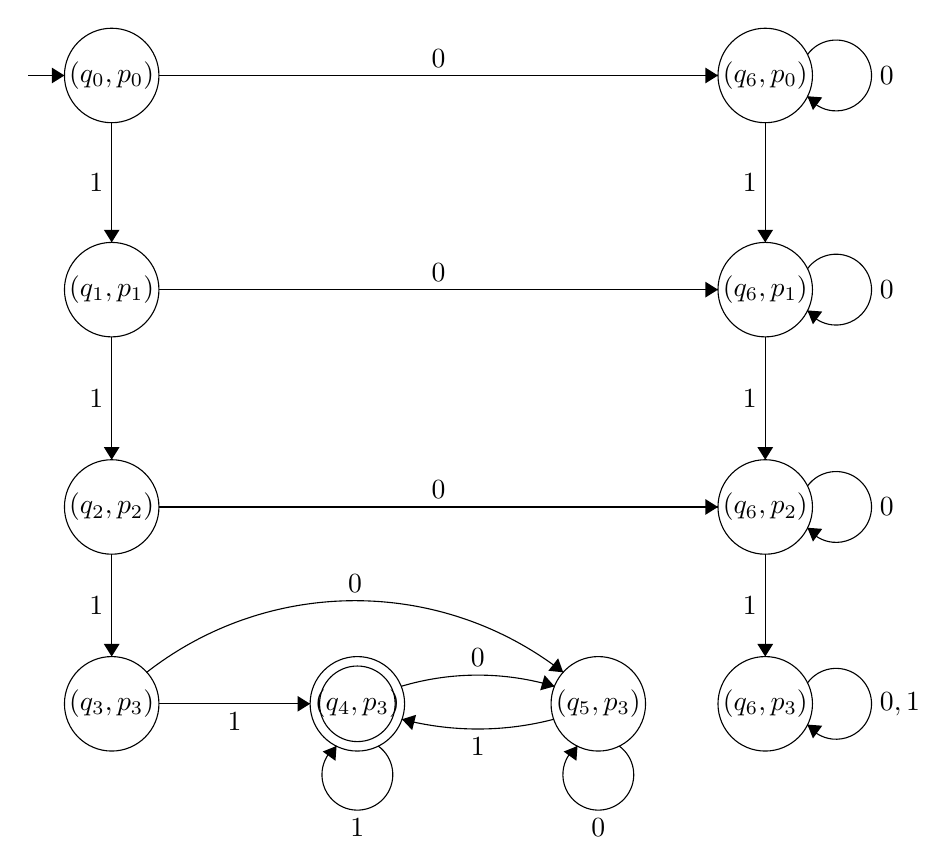
\begin{tikzpicture}[scale=0.2]
\tikzstyle{every node}+=[inner sep=0pt]
\draw [black] (21.1,-11) circle (3);
\draw (21.1,-11) node {$(q_0,p_0)$};
\draw [black] (62.6,-11) circle (3);
\draw (62.6,-11) node {$(q_6,p_0)$};
\draw [black] (21.1,-24.6) circle (3);
\draw (21.1,-24.6) node {$(q_1,p_1)$};
\draw [black] (62.6,-24.6) circle (3);
\draw (62.6,-24.6) node {$(q_6,p_1)$};
\draw [black] (21.1,-38.4) circle (3);
\draw (21.1,-38.4) node {$(q_2,p_2)$};
\draw [black] (62.6,-38.4) circle (3);
\draw (62.6,-38.4) node {$(q_6,p_2)$};
\draw [black] (21.1,-50.9) circle (3);
\draw (21.1,-50.9) node {$(q_3,p_3)$};
\draw [black] (36.7,-50.9) circle (3);
\draw (36.7,-50.9) node {$(q_4,p_3)$};
\draw [black] (36.7,-50.9) circle (2.4);
\draw [black] (52,-50.9) circle (3);
\draw (52,-50.9) node {$(q_5,p_3)$};
\draw [black] (62.6,-50.9) circle (3);
\draw (62.6,-50.9) node {$(q_6,p_3)$};
\draw [black] (15.8,-11) -- (18.1,-11);
\fill [black] (18.1,-11) -- (17.3,-10.5) -- (17.3,-11.5);
\draw [black] (24.1,-11) -- (59.6,-11);
\fill [black] (59.6,-11) -- (58.8,-10.5) -- (58.8,-11.5);
\draw (41.85,-10.5) node [above] {$0$};
\draw [black] (21.1,-14) -- (21.1,-21.6);
\fill [black] (21.1,-21.6) -- (21.6,-20.8) -- (20.6,-20.8);
\draw (20.6,-17.8) node [left] {$1$};
\draw [black] (65.28,-9.677) arc (144:-144:2.25);
\draw (69.85,-11) node [right] {$0$};
\fill [black] (65.28,-12.32) -- (65.63,-13.2) -- (66.22,-12.39);
\draw [black] (62.6,-14) -- (62.6,-21.6);
\fill [black] (62.6,-21.6) -- (63.1,-20.8) -- (62.1,-20.8);
\draw (62.1,-17.8) node [left] {$1$};
\draw [black] (24.1,-24.6) -- (59.6,-24.6);
\fill [black] (59.6,-24.6) -- (58.8,-24.1) -- (58.8,-25.1);
\draw (41.85,-24.1) node [above] {$0$};
\draw [black] (21.1,-27.6) -- (21.1,-35.4);
\fill [black] (21.1,-35.4) -- (21.6,-34.6) -- (20.6,-34.6);
\draw (20.6,-31.5) node [left] {$1$};
\draw [black] (65.28,-23.277) arc (144:-144:2.25);
\draw (69.85,-24.6) node [right] {$0$};
\fill [black] (65.28,-25.92) -- (65.63,-26.8) -- (66.22,-25.99);
\draw [black] (62.6,-27.6) -- (62.6,-35.4);
\fill [black] (62.6,-35.4) -- (63.1,-34.6) -- (62.1,-34.6);
\draw (62.1,-31.5) node [left] {$1$};
\draw [black] (24.1,-38.4) -- (59.6,-38.4);
\fill [black] (59.6,-38.4) -- (58.8,-37.9) -- (58.8,-38.9);
\draw (41.85,-37.9) node [above] {$0$};
\draw [black] (21.1,-41.4) -- (21.1,-47.9);
\fill [black] (21.1,-47.9) -- (21.6,-47.1) -- (20.6,-47.1);
\draw (20.6,-44.65) node [left] {$1$};
\draw [black] (65.28,-37.077) arc (144:-144:2.25);
\draw (69.85,-38.4) node [right] {$0$};
\fill [black] (65.28,-39.72) -- (65.63,-40.6) -- (66.22,-39.79);
\draw [black] (62.6,-41.4) -- (62.6,-47.9);
\fill [black] (62.6,-47.9) -- (63.1,-47.1) -- (62.1,-47.1);
\draw (62.1,-44.65) node [left] {$1$};
\draw [black] (23.329,-48.896) arc (127.94951:52.05049:21.498);
\fill [black] (49.77,-48.9) -- (49.45,-48.01) -- (48.83,-48.8);
\draw (36.55,-43.85) node [above] {$0$};
\draw [black] (24.1,-50.9) -- (33.7,-50.9);
\fill [black] (33.7,-50.9) -- (32.9,-50.4) -- (32.9,-51.4);
\draw (28.9,-51.4) node [below] {$1$};
\draw [black] (38.023,-53.58) arc (54:-234:2.25);
\draw (36.7,-58.15) node [below] {$1$};
\fill [black] (35.38,-53.58) -- (34.5,-53.93) -- (35.31,-54.52);
\draw [black] (39.483,-49.79) arc (106.67382:73.32618:16.963);
\fill [black] (49.22,-49.79) -- (48.59,-49.08) -- (48.31,-50.04);
\draw (44.35,-48.58) node [above] {$0$};
\draw [black] (49.169,-51.882) arc (-75.37336:-104.62664:19.082);
\fill [black] (39.53,-51.88) -- (40.18,-52.57) -- (40.43,-51.6);
\draw (44.35,-53) node [below] {$1$};
\draw [black] (53.323,-53.58) arc (54:-234:2.25);
\draw (52,-58.15) node [below] {$0$};
\fill [black] (50.68,-53.58) -- (49.8,-53.93) -- (50.61,-54.52);
\draw [black] (65.28,-49.577) arc (144:-144:2.25);
\draw (69.85,-50.9) node [right] {$0,1$};
\fill [black] (65.28,-52.22) -- (65.63,-53.1) -- (66.22,-52.29);
\end{tikzpicture}
\end{center}

Es wäre uns natürlich einiges an Kamalitäten erspart geblieben, wenn wir geschnallt hätten, dass
\[
L_3 - (\{0,1\}^* - L_1) = L_3 \cap L_1
\]

\end{document}
